%% LyX 2.2.2 created this file.  For more info, see http://www.lyx.org/.
%% Do not edit unless you really know what you are doing.
\documentclass[11pt,english]{article}
\renewcommand{\rmdefault}{cmr}
\renewcommand{\sfdefault}{cmss}
\renewcommand{\ttdefault}{cmtt}
\usepackage[T1]{fontenc}
\usepackage[latin9]{inputenc}
\usepackage{geometry}
\geometry{verbose,tmargin=2.5cm,bmargin=2.5cm,lmargin=2.5cm,rmargin=2.5cm}
\usepackage{babel}
\usepackage{amsmath}
\usepackage{amsthm}
\usepackage{amssymb}
\usepackage[unicode=true,pdfusetitle,
 bookmarks=true,bookmarksnumbered=false,bookmarksopen=false,
 breaklinks=false,pdfborder={0 0 0},pdfborderstyle={},backref=false,colorlinks=false]
 {hyperref}

\makeatletter
%%%%%%%%%%%%%%%%%%%%%%%%%%%%%% Textclass specific LaTeX commands.
\theoremstyle{plain}
\newtheorem{thm}{\protect\theoremname}[section]
  \theoremstyle{plain}
  \newtheorem{cor}[thm]{\protect\corollaryname}
  \theoremstyle{plain}
  \newtheorem{lem}[thm]{\protect\lemmaname}
  \theoremstyle{plain}
  \newtheorem{prop}[thm]{\protect\propositionname}
  \theoremstyle{plain}
  \newtheorem{conjecture}[thm]{\protect\conjecturename}
  \theoremstyle{definition}
  \newtheorem{defn}[thm]{\protect\definitionname}
  \theoremstyle{definition}
  \newtheorem{example}[thm]{\protect\examplename}
  \theoremstyle{remark}
  \newtheorem{rem}[thm]{\protect\remarkname}
  \theoremstyle{remark}
  \newtheorem{claim}[thm]{\protect\claimname}
  \theoremstyle{plain}
  \newtheorem{fact}[thm]{\protect\factname}
  \theoremstyle{definition}
  \newtheorem{sol}[thm]{\protect\solutionname}

%%%%%%%%%%%%%%%%%%%%%%%%%%%%%% User specified LaTeX commands.
\date{}

\usepackage{appendix}

% for better spacing on boldsymbol
\usepackage{bm}

% cleveref allows \ref{thm:asdf} instead of Theorem~\ref{thm:asdf}
\usepackage[nameinlink,capitalise,noabbrev]{cleveref}
\AtBeginDocument{\renewcommand{\ref}[1]{\cref{#1}}}
\crefname{appsec}{Appendix}{Appendices}
\creflabelformat{enumi}{#2textup{#1}#3}

%\usepackage[parfill]{parskip}
%\setlength{\parskip}{\bigskipamount}

%have space before theorems
%\begingroup
%    \makeatletter
%    \@for\theoremstyle:=definition,remark,plain\do{%
%        \expandafter\g@addto@macro\csname th@\theoremstyle\endcsname{%
%            \addtolength\thm@preskip\parskip
%            }%
%        }
%\endgroup

% LyX won't let me include cleveref before theorem declarations so I need to redefine everything as a hack
\theoremstyle{plain}
\newtheorem{mythm}{\protect\theoremname}[section]
\renewenvironment{thm}{\begin{mythm}}{\end{mythm}}
\crefname{mythm}{Theorem}{Theorems}
\theoremstyle{definition}
\newtheorem{mydefn}[mythm]{\protect\definitionname}
\renewenvironment{defn}{\begin{mydefn}}{\end{mydefn}}
\theoremstyle{definition}
\newtheorem{myfact}[mythm]{\protect\factname}
\renewenvironment{fact}{\begin{myfact}}{\end{myfact}}
\theoremstyle{definition}
\newtheorem{myexample}[mythm]{\protect\examplename}
\renewenvironment{example}{\begin{myexample}}{\end{myexample}}
\theoremstyle{plain}
\newtheorem{myprop}[mythm]{\protect\propositionname}
\renewenvironment{prop}{\begin{myprop}}{\end{myprop}}
\theoremstyle{plain}
\newtheorem{mycor}[mythm]{\protect\corollaryname}
\renewenvironment{cor}{\begin{mycor}}{\end{mycor}}
\theoremstyle{plain}
\newtheorem{mylem}[mythm]{\protect\lemmaname}
\renewenvironment{lem}{\begin{mylem}}{\end{mylem}}
\crefname{mylem}{Lemma}{Lemmas}
\theoremstyle{plain}
\newtheorem{myconjecture}{\protect\conjecturename}
\renewenvironment{conjecture}{\begin{myconjecture}}{\end{myconjecture}}
\theoremstyle{definition}
\newtheorem{myrem}[mythm]{\protect\remarkname}
\renewenvironment{rem}{\begin{myrem}}{\end{myrem}}
\theoremstyle{remark}
\newtheorem{myclaim}[mythm]{\protect\claimname}
\renewenvironment{claim}{\begin{myclaim}}{\end{myclaim}}
\theoremstyle{plain}
\newtheorem{myfakethm}[mythm]{``Theorem''}
\renewenvironment{sol}{\begin{myfakethm}}{\end{myfakethm}}
% equation cref format
\crefformat{equation}{#2(#1)#3}

% \left(\right) should behave the same as ()
\let\originalleft\left
\let\originalright\right
\renewcommand{\left}{\mathopen{}\mathclose\bgroup\originalleft}
\renewcommand{\right}{\aftergroup\egroup\originalright}
\usepackage{pgfplots}
\usetikzlibrary{pgfplots.groupplots}
\usepackage{verbatim}

%make sure tildes in url are vertically centered
\makeatletter
\renewcommand*{\UrlTildeSpecial}{%
  \do\~{%
    \mbox{%
      \fontfamily{ptm}\selectfont
      \textasciitilde
    }%
  }%  
}%    
\let\Url@force@Tilde\UrlTildeSpecial
\makeatother

%graph drawing
\usepackage{tikz}
%\usetikzlibrary{external}
%\usetikzlibrary{decorations.markings}
%\usetikzlibrary{arrows.meta}
%\tikzexternalize
\tikzstyle{vertex}=[circle,draw=black,fill=black,inner sep=0,minimum size=0.2cm,text=white,font=\footnotesize]
%\tikzset{arc/.style={
%        decoration={markings,
%            mark= at position 0.5 with {\arrow{Latex[length=2mm,width=2mm]}} ,
%        },
%        postaction={decorate}
%    }
%}
\tikzset{every loop/.style={min distance=50,in=50,out=130,looseness=7}}

%caption labels
\usepackage[labelfont=bf,labelsep=period]{caption}

\usepackage{enumitem}

\makeatother

  \providecommand{\claimname}{Claim}
  \providecommand{\conjecturename}{Conjecture}
  \providecommand{\corollaryname}{Corollary}
  \providecommand{\definitionname}{Definition}
  \providecommand{\examplename}{Example}
  \providecommand{\factname}{Fact}
  \providecommand{\lemmaname}{Lemma}
  \providecommand{\propositionname}{Proposition}
  \providecommand{\remarkname}{Remark}
\providecommand{\solutionname}{Solution}
\providecommand{\theoremname}{Theorem}

\begin{document}

\title{Almost all Steiner Triple Systems have perfect matchings}

\author{Matthew Kwan \thanks{Department of Mathematics, ETH, 8092 Z�rich. Email: \href{mailto:matthew.kwan@math.ethz.ch} {\nolinkurl{matthew.kwan@math.ethz.ch}}.}}

\maketitle
\global\long\def\RR{\mathbb{R}}

\global\long\def\QQ{\mathbb{Q}}

\global\long\def\HH{\mathbb{H}}

\global\long\def\E{\mathbb{E}}

\global\long\def\Var{\operatorname{Var}}

\global\long\def\CC{\mathbb{C}}

\global\long\def\NN{\mathbb{N}}

\global\long\def\ZZ{\mathbb{Z}}

\global\long\def\GG{\mathbb{G}}

\global\long\def\BB{\mathbb{B}}

\global\long\def\DD{\mathbb{D}}

\global\long\def\cL{\mathcal{L}}

\global\long\def\supp{\operatorname{supp}}

\global\long\def\one{\boldsymbol{1}}

\global\long\def\range#1{\left[#1\right]}

\global\long\def\d{\operatorname{d}}

\global\long\def\falling#1#2{\left(#1\right)_{#2}}

\global\long\def\f{\mathbf{f}}

\global\long\def\im{\operatorname{im}}

\global\long\def\sp{\operatorname{span}}

\global\long\def\rank{\operatorname{rank}}

\global\long\def\sign{\operatorname{sign}}

\global\long\def\mod{\operatorname{mod}}

\global\long\def\id{\operatorname{id}}

\global\long\def\disc{\operatorname{disc}}

\global\long\def\lindisc{\operatorname{lindisc}}

\global\long\def\tr{\operatorname{tr}}

\global\long\def\adj{\operatorname{adj}}

\global\long\def\Unif{\operatorname{Unif}}

\global\long\def\Po{\operatorname{Po}}

\global\long\def\Bin{\operatorname{Bin}}

\global\long\def\Ber{\operatorname{Ber}}

\global\long\def\Geom{\operatorname{Geom}}

\global\long\def\sat{\operatorname{sat}}

\global\long\def\Hom{\operatorname{Hom}}

\global\long\def\vol{\operatorname{vol}}

\global\long\def\floor#1{\left\lfloor #1\right\rfloor }

\global\long\def\ceil#1{\left\lceil #1\right\rceil }

\global\long\def\cond{\,\middle|\,}

\let\polishL\L

%\global\long\def\L{\mathcal{L}}

\DeclareRobustCommand{\L}{\ifmmode{\mathcal{L}}\else\polishL\fi}

\global\long\def\randS{\boldsymbol{S}}

\global\long\def\S{\mathcal{S}}

\global\long\def\Sm#1{\mathcal{S}_{#1}}

\global\long\def\ord{\mathcal{O}}

\global\long\def\ordm#1{\mathcal{O}_{#1}}

\global\long\def\cordm#1#2{\mathcal{O}_{#2}^{#1}}

\global\long\def\cSm#1#2{\mathcal{S}_{#2}^{#1}}

\global\long\def\ext#1{\mathcal{O}^{\mathrm{ext}}\left(#1\right)}

\global\long\def\randN{\boldsymbol{N}}

\global\long\def\randX{\boldsymbol{X}}

\global\long\def\rg#1#2{\RR\left(#1,#2\right)}

\global\long\def\Gnp#1#2{\GG\left(#1,#2\right)}

\global\long\def\GSnp#1#2{\GG^{*}\left(#1,#2\right)}

\global\long\def\randG{\boldsymbol{G}}

\global\long\def\randY{\boldsymbol{Y}}

\global\long\def\randZ{\boldsymbol{Z}}

\global\long\def\randM{\boldsymbol{M}}

\global\long\def\randL{\boldsymbol{L}}

\begin{comment}
\begin{thm}
t
\end{thm}
\begin{cor}
c
\end{cor}
\begin{lem}
l
\end{lem}
\begin{prop}
p
\end{prop}
\begin{conjecture}
c
\end{conjecture}
\begin{defn}
d
\end{defn}
\begin{example}
e
\end{example}
\begin{rem}
r
\end{rem}
\begin{claim}
c
\end{claim}
\begin{fact}
f
\end{fact}
\begin{sol}
s
\end{sol}
\end{comment}
\begin{abstract}
We show that for any $n$ divisible by 3, almost all order-$n$ Steiner
triple systems have a perfect matching (also known as a parallel class).
In fact, we prove a general upper bound on the number of perfect matchings
in a Steiner triple system and show that almost all Steiner triple
systems essentially attain this maximum. We accomplish this via a
general theorem comparing a uniformly random Steiner triple system
to the outcome of the triangle removal process, which we hope will
be useful for other problems. We believe our methods can be easily
adapted to other types of designs, for example to show that almost
all Latin squares have transversals.
\end{abstract}

\section{Introduction}

A \emph{Steiner triple system} of order $n$ is a collection $S$
of size-$3$ subsets of $\range n=\left\{ 1,\dots,n\right\} $ (that
is, a $3$-uniform hypergraph on the vertex set $\range n$), such
that every pair of vertices is included in exactly one hyperedge of
$S$. Steiner triple systems are among the most fundamental types
of combinatorial designs, and have strong connections to a wide range
of different subjects, ranging from group theory, to finite geometry,
to experimental design, to the theory of error-correcting codes. See
\cite{CR99} for an introduction to the subject. We note that a Steiner
triple system is actually nothing more than a triangle-decomposition
of the edges of the complete graph $K_{n}$, so Steiner triple systems
are natural ``symmetric'' counterparts to \emph{Latin squares},
which can be defined as triangle-decompositions of the complete tripartite
graph $K_{n,n,n}$.

In 1974 Wilson \cite{Wil74} used estimates for the number of Latin
squares to prove a coarse estimate for the number of Steiner triple
systems. Babai \cite{Bab80} used this estimate to prove that a $\left(1-o\left(1\right)\right)$-proportion
of Steiner triple systems have trivial automorphism group (equivalently,
a uniformly random order-$n$ Steiner triple system a.a.s.\footnote{By ``asymptotically almost surely'', or ``a.a.s.'', we mean that
the probability of an event is $1-o\left(1\right)$. Here and for
the rest of the paper, asymptotics are as $n\to\infty$.} has trivial automorphism group). We believe this is the only nontrivial
property known to hold a.a.s. for random Steiner triple systems. Following
Erd\H os and R\'enyi's seminal paper \cite{ER59} on random graphs
and Erd\H os' popularization of the probabilistic method, there have
been great developments in the theory of random combinatorial structures
of all kinds, but essentially none of the tools developed seem to
be applicable to Steiner triple systems. Steiner triple systems lack
independence or any kind of recursive structure, which rules out many
of the techniques used to study Erd\H os-R\'enyi random graphs and
random permutations, and there is basically no freedom to make local
changes, which precludes the use of ``switching'' techniques often
used in the study of random regular graphs (see for example \cite{KSVW01}).
It is not even clear how to study random Steiner triple systems empirically;
in an attempt to find an efficient algorithm to generate a random
Steiner triple system, Cameron \cite{Cam02} designed a Markov chain
on Steiner triple systems, but he was not able to determine whether
this chain was connected.

In a huge breakthrough that will surely revolutionize design theory,
Keevash \cite{Kee14} very recently proved that for a large class
of combinatorial designs generalizing Steiner triple systems, ``partial''
designs satisfying a certain ``quasirandomness'' condition can be
completed into designs. Shortly afterwards \cite{Kee15}, he showed
that his results could be used for approximate enumeration; in particular,
matching an upper bound due to Linial and Luria \cite{LL13} he proved
that there are
\begin{equation}
\left(n/e^{2}+o\left(n\right)\right)^{n^{2}/6}\label{eq:num-STS}
\end{equation}
Steiner triple systems of order $n$, as long as $n$ satisfies a
necessary divisibility condition (Steiner triple systems can only
exist if $n$ is 1 or 3 mod 6).

Of course, this new estimate makes it possible, in theory, to prove
new a.a.s. properties of random Steiner triple systems just by giving
an estimate asymptotically smaller than \ref{eq:num-STS} for the
number of Steiner triple systems not satisfying a certain property.
However, for most properties it is not at all clear how to prove such
estimates. Instead, we introduce a way to use Keevash's methods to
show that a uniformly random Steiner triple system can in some sense
be approximated by the outcome of a random process called the \emph{triangle
removal process}. We remark that actually Keevash's lower bound is
proved via a randomized construction that involves the triangle removal
process, so many properties that hold a.a.s. in the triangle removal
process trivially hold a.a.s. in this random construction. Such results
have been proved in \cite[Proposition~3.1]{LL15} and \cite{LLR15}.
However, the Steiner triple systems obtainable by Keevash's construction
comprise a negligible proportion of the set of Steiner triple systems,
so a more delicate approach is required to study a uniformly random
Steiner triple system. We give the details in \ref{sec:outline}.

As an application of our new method, we prove that if $3\mid n$ (that
is, if $n\equiv3\mod6$) then almost all order-$n$ Steiner triple
systems have many \emph{perfect matchings}. A perfect matching in
a hypergraph is a collection of disjoint hyperedges partitioning the
vertex set. The existence of perfect matchings is one of the most
central questions in the theory of graphs and hypergraphs; in particular,
one of the most celebrated recent developments in the field is the
Fulkerson-prize-winning work of Johansson, Kahn and Vu \cite{JKV08}
on perfect matchings in random hypergraphs. A perfect matching in
a Steiner triple system is also called a\emph{ parallel class}, and
has particular significance. One of the oldest problems in combinatorics,
famously solved by Ray-Chaudhuri and Wilson \cite{RW71}, asks whether
for all $n\equiv3\mod6$ there exists an order-$n$  Steiner triple
system which can be partitioned into hyperedge-disjoint perfect matchings
(a \emph{Kirkman triple system}). Alon, Kim and Spencer \cite{AKS97}
proved that every Steiner triple system has an almost-perfect matching
covering all but $o\left(\sqrt{n}\log^{3/2}n\right)$ vertices, and
Bryant and Horsley \cite{BH15} proved that for infinitely many $n\equiv3\mod6$
there exist Steiner triple systems with no perfect matching.
\begin{thm}
\label{thm:PM-in-STS}Let $n\equiv3\mod6$ and let $\randS$ be a
uniformly random order-$n$ Steiner triple system. Then a.a.s. $\randS$
contains
\[
\left(\left(1-o\left(1\right)\right)\frac{n}{2e^{2}}\right)^{n/3}
\]
perfect matchings.
\end{thm}
We remark that if $3\nmid n$ (that is, if $n\equiv1\mod6$) then
obviously no order-$n$ Steiner triple system can have a perfect matching,
but exactly the same proof can be used to show that there is a matching
covering all but one vertex.

We prove \ref{thm:PM-in-STS} in \ref{sec:absorbers} using our new
method combined with the so-called \emph{absorbing method}, which
was introduced as a general method by R\"odl, Ruci\'nski and Szemer\'edi
\cite{RRS09} (though the basic idea had been used earlier, for example
by Krivelevich \cite{Kri97}). Basically, we prove the a.a.s. existence
of certain small substructures that allow us to complete an almost-perfect
matching into a perfect one.

Up to the error term, a random Steiner triple system actually has
the maximum possible number of perfect matchings: we also prove the
following upper bound.
\begin{thm}
\label{thm:maximum-PMs}Any Steiner triple system has at most
\[
\left(\left(1+o\left(1\right)\right)\frac{n}{2e^{2}}\right)^{n/3}
\]
perfect matchings.
\end{thm}
We give a short proof of \ref{thm:maximum-PMs} in \ref{sec:max-num-matchings},
using the so-called \emph{entropy method} due to Radhakrishnan \cite{Rad97}.

\subsection{Latin squares}

An order-$n$ Latin square is usually defined as an $n\times n$ array
of the numbers between 1 and $n$ (we call these \emph{symbols}),
such that each row and column contains each symbol exactly once. As
mentioned earlier, this is equivalent to a 3-uniform hypergraph whose
triples comprise a triangle-decomposition of the edges of the complete
tripartite graph $K_{n,n,n}$ (the three parts correspond to the rows,
columns and symbols, so a triangle $\left(i,j,k\right)$ corresponds
to putting the symbol $k$ in the cell $\left(i,j\right)$). A perfect
matching in a Latin square is called a \emph{transversal }and the
property of containing a transversal is of great interest. In particular,
the famous Ryser-Brualdi-Stein conjecture speculates that every odd-order
Latin square has a transversal, and every even-order Latin square
has a partial transversal (matching) of size $n-1$. See the survey
of Wanless \cite{Wan11} for more information.

We are quite confident that our methods can be adapted to the setting
of Latin squares. The main obstacle is that Keevash's completion results
have not yet been adapted to Latin squares. We believe such an adaptation
should be quite straightforward, but it would be well outside the
scope of this paper to include the details here. Modulo a Keevash-type
completion result we can prove the following theorem, answering a
question of Glebov and Luria \cite{GL16} and proving that the Ryser-Brualdi-Stein
conjecture holds for almost all Latin squares.
\begin{sol}
\label{thm:latin}Let $\randL$ be a uniformly random order-$n$ Latin
square. Then a.a.s. $\randL$ contains
\[
\left(\left(1-o\left(1\right)\right)\frac{n}{e^{2}}\right)^{n}
\]
transversals.
\end{sol}
We note that the counterpart of \ref{thm:maximum-PMs} for Latin squares
(that a Latin square can have at most $\left(\left(1+o\left(1\right)\right)n/e^{2}\right)^{n}$
transversals) was first proved by Taranenko \cite{Tar15}. In \ref{sec:latin}
we outline how the proof of \ref{thm:PM-in-STS} can be adapted to
prove \ref{thm:latin}, conditional on a Keevash-type completion result.

\subsection{Structure of the paper}

The structure of this paper is as follows. In \ref{sec:outline} we
explain our method for studying random Steiner triple systems. In
\ref{sec:absorbers} we define absorbers and prove \ref{thm:PM-in-STS},
in \ref{sec:max-num-matchings} we prove \ref{thm:maximum-PMs}, and
in \ref{sec:latin} we sketch how \ref{thm:latin} may be proved.
In \ref{sec:concluding} we have some concluding remarks, including
a long list of open problems. Finally, we have two appendices; in
\ref{sec:keevash} we provide a straightforward but necessary adaptation
of Keevash's proof of \ref{eq:num-STS}, to estimate the number of
completions of a partial Steiner triple system, and in \ref{sec:Random-triangle-removal}
we have a very simple analysis of the triangle removal process.

\subsection{Acknowledgements}

The author would like to thank Asaf Ferber and Benny Sudakov for very
helpful discussions about random designs and the intricacies of the
absorbing method. Asaf and Benny could both have deservedly been coauthors
on this paper, but graciously declined the opportunity.

\section{\label{sec:outline}Random Steiner triple systems via the triangle
removal process}

In this section we describe our method for comparing random Steiner
triple systems with the outcome of the triangle removal process. Let
$N={n \choose 2}/3=\left(1+o\left(1\right)\right)n^{2}/6$ be the
number of hyperedges in a Steiner triple system. We also assume throughout
this section that $n$ is 1 or 3 mod 6.

We will shortly state a general theorem for comparing Steiner triple
systems with the triangle removal processes, but first we need several
definitions.
\begin{defn}[partial systems]
A \emph{partial Steiner triple system} (or \emph{partial system}
for short) is a $3$-uniform hypergraph on $\range n$ in which every
pair of vertices is included in no more than one hyperedge. Let $\Sm m$
be the set of partial systems with $m$ hyperedges. We will also want
to consider partial systems equipped with an ordering on their hyperedges.
Let $\ord$ be the set of ordered Steiner triple systems, and let
$\ordm m$ be the set of ordered partial systems with $m$ hyperedges.
For $S\in\ordm m$ and $i\le m$, let $S_{i}$ be the partial system
consisting of the first $i$ hyperedges of $S$. For a (possibly ordered)
partial system $S$, let $G\left(S\right)$ be the graph with an edge
for every pair of vertices which does not\emph{ }appear in any hyperedge
of $S$. So, if $S$ has $m$ hyperedges, then $G\left(S\right)$
has ${n \choose 2}-3m$ edges.
\end{defn}
%
\begin{defn}[quasirandomness]
For a graph $G$ with $m$ edges, let $d\left(G\right)=m/{n \choose 2}$
denote its density. We say $G$ is \emph{$\left(\varepsilon,h\right)$-quasirandom}
if for every set $A$ of at most $h$ vertices, we have $\left|\bigcap_{w\in A}N_{G}\left(w\right)\right|=\left(1\pm\varepsilon\right)d\left(G\right)^{\left|A\right|}n$.
(The notation $f=1\pm\varepsilon$ means $1-\varepsilon\le f\le1+\varepsilon$).
Let $\cSm{\varepsilon,h}m\subseteq\Sm m$ be the set of partial systems
$S\in\Sm m$ such that $G\left(S\right)$ is $\left(\varepsilon,h\right)$-quasirandom,
and let $\cordm{\varepsilon,h}m\subseteq\ordm m$ be the set of ordered
partial systems $S\in\ordm m$ such that $S_{i}\in\cSm{\varepsilon,h}i$
for each $i\le m$.
\end{defn}
%
\begin{defn}[the triangle removal processs]
The triangle removal process is defined as follows. Start with the
complete graph $K_{n}$ and iteratively delete a triangle chosen uniformly
at random from all triangles in the remaining graph. If we continue
this process for $m$ steps, the deleted triangles (in order) can
be interpreted as an ordered partial system in $\ordm m$. It is also
possible that the process aborts (because there are no triangles left)
before $m$ steps, in which case we say it returns the value ``$*$''.
We denote by $\rg nm$ the resulting distribution on $\ordm m\cup\left\{ *\right\} $.
\end{defn}
Now, our general theorem is as follows.
\begin{thm}
\label{lem:triangle-removal-transfer}There is $h_{0}\in\NN$ such
that for fixed $h\ge h_{0}$ and sufficiently small $a$ there is
$b\left(a\right)>0$ such that the following holds. Fix $\alpha\in\left(0,1\right)$,
let $\mathcal{P}\subseteq\ordm{\alpha N}$ be a property of ordered
partial systems, let $\mathcal{Q}\supseteq\cordm{n^{-a},h}{\alpha N}$,
let $\randS\in\ord$ be uniformly random and let $\randS'\in\rg n{\alpha N}$.
If
\[
\Pr\left(\randS'\notin\mathcal{P}\cond\randS'\in\mathcal{Q}\right)\le\exp\left(-n^{2-b}\right)
\]
then
\[
\Pr\left(\randS_{\alpha N}\notin\mathcal{P}\right)\le\exp\left(-\Omega\left(n^{1-2a}\right)\right).
\]
\end{thm}
Note that (as we prove in \ref{sec:Random-triangle-removal}), the
triangle removal process is likely to produce quasirandom graphs;
that is, $\Pr\left(\randS'\in\mathcal{Q}\right)=1-o\left(1\right)$.
However, as we will see in \ref{subsec:absorbers}, the conditioning
in \ref{lem:triangle-removal-transfer} can still be useful because
the probabilities under consideration are so small (it is certainly
not true that $\Pr\left(\randS'\notin\mathcal{Q}\right)$ is anywhere
near as small as $\exp\left(-\Omega\left(n^{2}\right)\right)$).

\begin{comment}

\textbf{TODO: work out the dependence on $\alpha$ so \ref{lem:triangle-removal-transfer}
can be used for $\alpha$ non-constant}

\end{comment}

The proof of \ref{lem:triangle-removal-transfer} follows from a sequence
of several lemmas. The most important is the following: we can use
Keevash's methods to estimate the number of ways to complete any $S\in\cordm{\varepsilon,h}{\alpha N}$,
and show that it does not vary too much between choices of $S$.
\begin{lem}
\label{prop:num-extensions}There is $h\in\NN$ such that for any
fixed $a>0$, there is $b=b\left(a\right)>0$ such that the following
holds. For any fixed $\alpha\in\left(0,1\right)$, any $\varepsilon\le n^{-a}$,
and any $S,S'\in\cordm{\varepsilon,h}{\alpha N}$,
\[
\frac{\left|\ext S\right|}{\left|\ext{S'}\right|}\le\exp\left(n^{2-b}\right).
\]
\end{lem}
\ref{prop:num-extensions} can be proved with only very slight adaptations
to the proof of \ref{eq:num-STS} in \cite{Kee15}. The details are
in \ref{sec:keevash}. The point of \ref{prop:num-extensions} is
that if we can prove some property holds with extremely high probability
(say $1-\exp\left(-\Omega\left(n^{2}\right)\right)$) in a uniformly
random $\randS\in\cordm{\varepsilon,h}{\alpha N}$, then it also holds
with essentially the same probability in $\randS_{\alpha N}$, for
a uniformly random $\randS\in\ord$ conditioned on the event $\randS_{\alpha N}\in\cordm{\varepsilon,h}{\alpha N}$.

The next step is to show that the event $\randS_{\alpha N}\in\cordm{\varepsilon,h}{\alpha N}$
is very likely. In fact, this event occurs a.a.s. for a random ordering
of any given Steiner triple system. We prove the following lemma in
\ref{sec:random-is-typical}.
\begin{lem}
\label{lem:random-is-typical}The following holds for any fixed $h\in\NN$,
$\alpha\in\left(0,1\right)$ and $a\in\left(0,1/2\right)$. Let $\varepsilon=n^{-a}$,
consider any Steiner triple system $S$, and uniformly at random order
its hyperedges to obtain an ordered Steiner triple system $\randS\in\ord$.
Then $\Pr\left(\randS_{\alpha N}\notin\cordm{\varepsilon,h}{\alpha N}\right)=\exp\left(-\Omega\left(n^{1-2a}\right)\right)$.
\end{lem}
Therefore, if we can prove a property holds with extremely high probability
in a uniformly random $\randS\in\cordm{\varepsilon,h}{\alpha N}$
for sufficiently small $\varepsilon$ and sufficiently large $h$,
then that property also holds a.a.s. in the first $\alpha N$ edges
of a uniformly random $\randS\in\ord$.

Next, the following lemma says that each $S\in\cordm{\varepsilon,h}{\alpha N}$
is roughly equally likely to be produced by the triangle removal process,
so that $\RR\left(n,\alpha N\right)$ approximates the uniform distribution
on $S\in\cordm{\varepsilon,h}{\alpha N}$. It is proved in \ref{sec:greedy-random-approx-uniform}.
\begin{lem}
\label{lem:greedy-random-approx-uniform}For any $a>0$ and $\alpha\in\left[0,1\right]$,
and for $S,S'\in\cordm{n^{-a},2}{\alpha N}$ and $\randS\in\rg n{\alpha N}$,
\[
\frac{\Pr\left(\randS=S\right)}{\Pr\left(\randS=S'\right)}\le\exp\left(O\left(n^{2-a}\right)\right).
\]
\end{lem}
We can finally combine everything to prove \ref{lem:triangle-removal-transfer}.
\begin{proof}[Proof of \ref{lem:triangle-removal-transfer}]
We have
\begin{align*}
\Pr\left(\randS_{\alpha N}\notin\mathcal{P}\right) & \le\Pr\left(\randS_{\alpha N}\notin\mathcal{P}\cond\randS_{\alpha N}\in\cordm{n^{-a},h}{\alpha N}\right)+\Pr\left(\randS_{\alpha N}\notin\cordm{n^{-a},h}{\alpha N}\right)\\
 & \le\exp\left(O\left(n^{2-c}\right)\right)\Pr\left(\randS'\notin\mathcal{P}\cond\randS'\in\cordm{n^{-a},h}{\alpha N}\right)+\exp\left(-\Omega\left(n^{1-2a}\right)\right),
\end{align*}
where $c=b\left(a\right)$ in the notation of \ref{prop:num-extensions}.
But, if $a$ is small enough then \ref{lem:triangle-removal-analysis}
guarantees that $\Pr\left(\randS'\in\cordm{n^{-a},h}{\alpha N}\right)=1-o\left(1\right)$
so
\[
\Pr\left(\randS'\notin\mathcal{P}\cond\randS'\in\cordm{n^{-a},h}{\alpha N}\right)\le\Pr\left(\randS'\notin\mathcal{P}\cond\randS'\in\mathcal{Q}\right)\frac{\Pr\left(\randS'\in\mathcal{Q}\right)}{\Pr\left(\randS'\in\cordm{n^{-a},h}{\alpha N}\right)}=\left(1+o\left(1\right)\right)\Pr\left(\randS'\notin\mathcal{P}\cond\randS'\in\mathcal{Q}\right).
\]
If $b<c$ this completes the proof.
\end{proof}
In \ref{sec:random-is-typical} we prove \ref{lem:random-is-typical}
and in \ref{sec:greedy-random-approx-uniform} we prove \ref{lem:greedy-random-approx-uniform}.
Also, in \ref{lem:bite-transfer} we prove some lemmas which are useful
tools for applying \ref{lem:triangle-removal-transfer} in practice.

\subsection{Randomly ordered Steiner triple systems\label{sec:random-is-typical}}

In this subsection we prove \ref{lem:random-is-typical}.
\begin{proof}
Fix $m\le\alpha N$. Note that $\randS_{m}$ (as an unordered partial
system) is a uniformly random subset of $m$ hyperedges of $S$. We
can obtain an almost equivalent random partial system by including
each hyperedge of $S$ with independent probability $m/N$. Let $\randS'$
denote the partial system so obtained, and let $\randG'=G\left(\randS'\right)$.
Now, fix a set $A$ of at most $h$ vertices. It suffices to prove
\begin{align}
\left|\bigcap_{w\in A}N_{\randG'}\left(w\right)\right| & =\left(1+O\left(n^{-a}\right)\right)\left(1-\frac{m}{N}\right)^{\left|A\right|}n,\label{eq:degree-random-binomial}
\end{align}
with probability $1-\exp\left(-\Omega\left(n^{1-2a}\right)\right)$.
Indeed, the so-called Pittel inequality (see \cite[p.~17]{JLR00})
would imply that the same estimate holds with essentially the same
probability if we replace $\randS'$ with $\randS_{m}$, and then
we can apply the union bound over all $m\le\alpha N$ and all choices
of $A$.

Note that there are at most ${\left|A\right| \choose 2}=O\left(1\right)$
hyperedges of $S$ that include more than one vertex in $A$ (by the
defining property of a Steiner triple system). Let $U$ be the set
of vertices involved in these atypical hyperedges, plus the vertices
that appear in sets in $A$, so that $\left|U\right|=O\left(1\right)$.
Let $\randN=\left|\left(\bigcap_{w\in A}N_{\randG'}\left(w\right)\right)\backslash U\right|$.
For every $v\notin U$ and $w\in A$ there is exactly one hyperedge
$e_{v}^{w}$ in $S$ containing $v$ and $w$, whose presence in $\randS'$
would prevent $v$ from contributing to $\randN$. For each $v\notin U$
the hyperedges $e_{v}^{w}$ are distinct, so
\[
\Pr\left(v\in\bigcap_{w\in A}N_{\randG'}\left(w\right)\right)=\left(1-\frac{m}{N}\right)^{\left|A\right|},
\]
and by linearity of expectation $\E\randN=\left(1-m/N\right)^{\left|A\right|}\left(n-O\left(1\right)\right)$.
Now, $\randN$ is determined by the presence of at most $\left(n-\left|U\right|\right)\left|A\right|=O\left(n\right)$
hyperedges in $\randS'$, and changing the presence of each affects
$\randN$ by at most $2=O\left(1\right)$. So, by the Azuma-Hoeffding
inequality (see \cite[Section~2.4]{JLR00}),
\begin{align*}
\Pr\left(\left|\randN-\left(1-\frac{m}{N}\right)^{\left|A\right|}n\right|>n^{-a}\left(1-\frac{m}{N}\right)^{\left|A\right|}n\right) & \le\exp\left(-\Omega\left(\frac{\left(n^{-a}\left(1-\alpha\right)^{h}n\right)^{2}}{n}\right)\right)\\
 & =\exp\left(-\Omega\left(n^{1-2a}\right)\right).
\end{align*}
Finally, we recall that $\left|\left(\bigcap_{x\in X}N_{\randG'}\left(x\right)\right)\right|=\randN+O\left(1\right)$,
which completes the proof of \ref{eq:degree-random-binomial}.
\end{proof}

\subsection{Approximate uniformity of the triangle removal process\label{sec:greedy-random-approx-uniform}}

In this subsection we prove \ref{lem:greedy-random-approx-uniform}.
We first make a simple observation about small subgraph statistics
in quasirandom hypergraphs, which we will use at several points in
the paper.
\begin{prop}
\label{lem:H-count}Let $H$ be a fixed graph with an identified vertex
subset $U$, and let $\left|\operatorname{Aut}\left(H,U\right)\right|$
be the number of automorphisms of $H$ fixing $U$. Let $G$ be an
$\left(\varepsilon,v\left(H\right)-1\right)$-quasirandom graph on
$n$ vertices, and let $F$ be a copy of the induced graph $H\left[U\right]$
in $G$. Then, the number of completions of $F$ to a copy of $H$
is 
\[
\left(1\pm O\left(\varepsilon\right)\right)\left(1-\frac{i}{N}\right)^{e\left(H\right)-e\left(F\right)}\frac{n^{v\left(H\right)-\left|U\right|}}{\left|\operatorname{Aut}\left(H,U\right)\right|}.
\]
In particular, the number of copies of $H$ in $G$ is 
\[
\left(1\pm O\left(\varepsilon\right)\right)\left(1-\frac{i}{N}\right)^{e\left(H\right)}\frac{n^{v\left(H\right)}}{\left|\operatorname{Aut}\left(H\right)\right|}.
\]
\end{prop}
\begin{proof}
It suffices to show that the number of embeddings of $H$ (as a labelled
object) into $G$ extending $F$ is
\[
\left(1\pm O\left(\varepsilon\right)\right)\left(1-\frac{i}{N}\right)^{e\left(H\right)-e\left(F\right)}n^{v\left(H\right)-\left|U\right|}.
\]
We prove this by induction on the number of vertices in $V\left(H\right)\backslash U$.
The base case is where $U=V\left(H\right)$, which is trivial. Fix
a vertex $v\in V\left(H\right)\backslash U$; by induction there are
\[
\left(1\pm O\left(\varepsilon\right)\right)\left(1-\frac{i}{N}\right)^{e\left(H\right)-e\left(F\right)-d_{H}\left(v\right)}n^{v\left(H\right)-\left|U\right|-1}
\]
embeddings of $H-v$ extending $F$. For each such embedding, by $\left(\varepsilon,v\left(H\right)-1\right)$-quasirandomness,
there are $\left(1\pm\varepsilon\right)\left(1-\frac{i}{N}\right)^{d_{H}\left(v\right)}n$
ways to choose a vertex of $G$ with the right adjacencies to complete
the embedding of $H$.
\end{proof}
Now we are ready to prove \ref{lem:greedy-random-approx-uniform}.
\begin{proof}
Each $G\left(S_{i}\right)$ has 
\[
\left(1\pm O\left(n^{-a}\right)\right)\left(1-\frac{i}{N}\right)^{3}\frac{n^{3}}{6}
\]
triangles, by $\left(n^{-a},2\right)$-quasirandomness and \ref{lem:H-count}.
We therefore have
\[
\Pr\left(\randS=S\right)=\prod_{i=0}^{\alpha N-1}\frac{1}{\left(1\pm O\left(n^{-a}\right)\right)\left(1-i/N\right)^{3}n^{3}/6},
\]
and a similar expression holds for $\Pr\left(\randS=S'\right)$. Taking
quotients term-by-term gives
\begin{align*}
\frac{\Pr\left(\randS=S\right)}{\Pr\left(\randS=S'\right)} & \le\left(1+O\left(n^{-a}\right)\right)^{\alpha N}\\
 & \le\exp\left(O\left(n^{2-a}\right)\right)
\end{align*}
as desired.
\end{proof}

\subsection{A coupling lemma and a concentration inequality\label{sec:nibble-TRP-coupling}}

In this subsection we prove two lemmas that will be useful in combination
with \ref{lem:triangle-removal-transfer}. First, after some necessary
definitions we will show how to couple the triangle removal process
with a simpler random hypergraph distribution.
\begin{defn}
For a partial system $S$, let $\Gnp Sp$ be the random distribution
on $3$-uniform hypergraphs where each hyperedge not conflicting with
$S$ (that is, not intersecting a hyperedge of $S$ in more than $2$
vertices) is included with probability $p$. So, if $\varnothing$
is the empty order-$n$ partial system, then $\Gnp{\varnothing}p:=\Gnp np$
is the standard binomial random 3-graph. Let $\GSnp Sp$ be the distribution
on partial systems obtained from $\Gnp Sp$ by considering all hyperedges
which intersect another hyperedge in more than $2$ vertices, and
deleting all these hyperedges. Let $\rg Sm$ be the partial system
distribution obtained with $m$ steps of the triangle removal process
starting from $G\left(S\right)$.
\end{defn}
Note that ${n \choose 3}/n=\left(1+o\left(1\right)\right)N$. For
small $\alpha>0$, we can view $\GSnp S{\alpha/n}$ as a ``bite''
of a ``nibbling'' process (see for example \cite[Section~4.7]{AS04}),
that should be similar to $\rg S{\alpha N}$.
\begin{lem}
\label{lem:bite-transfer}let $\mathcal{P}$ be a property of unordered
partial systems that is monotone increasing in the sense that $S\in\mathcal{P}$
and $S'\supseteq S$ implies $S'\in\mathcal{P}$. For fixed $h\ge2$
and $a\in\left(0,1\right)$ there is $b\left(a,h\right)>0$ such that
the following holds. Fix $\alpha\in\left(0,1\right)$ and $S\in\cordm{n^{-a},h}m$
for some $m\le N-\alpha N$ and let $\mathcal{Q}=\left\{ S\in\cordm{n^{-b},h}{\alpha N+m}:S_{m}\in\cordm{n^{-a},h}m\right\} \supseteq\cordm{n^{-a},h}{\alpha N+m}$.
Let $\randS\in\rg S{\alpha N}$ and $\randS^{*}\in\GSnp S{\alpha/n}$.
Then
\[
\Pr\left(S\cup\randS\notin\mathcal{P}\cond S\cup\randS\in\mathcal{Q}\right)=O\left(1\right)\Pr\left(S\cup\randS^{*}\notin\mathcal{P}\right).
\]
\end{lem}
\begin{proof}
Let $\randS^{*}\in\GSnp S{\alpha/n}$ be obtained from $\randG\in\Gnp S{\alpha/n}$.
Note that conditioning on the number of edges in $\randG$, its edges
comprise a uniformly random subset of its size, of the set of all
possible edges. With probability $\Omega\left(1\right)$ the number
of edges in $\randG$ is at most ${n \choose 3}\alpha/n\le\alpha N$,
in which case $\randS^{*}$ can be coupled as a subset of $\randS$.
Indeed, a random ordering of $\randG$ can be viewed as the first
few elements of a random ordering of the set of all possible edges,
and the triangle removal process with this ordering produces a superset
of $\randS^{*}$.

Now, let $b$ be $a\,b\left(a,h\right)$ in the notation of \ref{lem:triangle-removal-analysis},
so that $\Pr\left(S\cup\randS\in\mathcal{Q}\right)=1-o\left(1\right)$.
We have
\begin{align*}
\Pr\left(S\cup\randS\notin\mathcal{P}\cond S\cup\randS\in\mathcal{Q}\right) & \le\Pr\left(S\cup\randS^{*}\notin\mathcal{P}\cond S\cup\randS\in\mathcal{Q}\text{ and }e\left(\randG\right)\le\alpha N\right)\\
 & \le\Pr\left(S\cup\randS^{*}\notin\mathcal{P}\right)/\Pr\left(S\cup\randS\in\mathcal{Q}\text{ and }e\left(\randG\right)\le\alpha N\right)\\
 & =\Pr\left(S\cup\randS^{*}\notin\mathcal{P}\right)/\Omega\left(1\right).\tag*{\qedhere}
\end{align*}
\end{proof}
In this subsection we also state and prove a bounded-differences inequality
with Bernstein-type tails which can be used to analyse $\GSnp S{\alpha/n}$.
Standard bounded-difference inequalities such as the Azuma-Hoeffding
inequality do not provide strong enough tail bounds to apply \ref{lem:triangle-removal-transfer}.
\begin{thm}
\label{thm:bernstein-type}Let $\boldsymbol{\omega}=\left(\boldsymbol{\omega}_{1},\dots,\boldsymbol{\omega}_{n}\right)$
be a sequence of independent, identically distributed random variables
with $\Pr\left(\boldsymbol{\omega}_{i}=1\right)=p$ and $\Pr\left(\boldsymbol{\omega}_{i}=0\right)=1-p$.
Let $f\left(\boldsymbol{\omega}\right)$ satisfy the Lipschitz condition
$\left|f\left(\boldsymbol{\omega}\right)-f\left(\boldsymbol{\omega}'\right)\right|\le K$
for all pairs $\boldsymbol{\omega},\boldsymbol{\omega}'\in\left\{ 0,1\right\} ^{n}$
differing in exactly one coordinate. Then
\[
\Pr\left(\left|f\left(\boldsymbol{\omega}\right)-\E f\left(\boldsymbol{\omega}\right)\right|>t\right)\le\exp\left(-\frac{t^{2}}{4K^{2}np+2Kt}\right).
\]
\end{thm}
\begin{proof}
We use Freedman's inequality (\ref{lem:freedman}), with the Doob
martingale $\randX\left(0\right),\dots,\randX\left(n\right)$ defined
by $\boldsymbol{X}\left(i\right)=\E\left[f\left(\boldsymbol{\omega}\right)\cond\boldsymbol{\omega}_{1},\dots,\boldsymbol{\omega}_{i}\right]$.
Note that $\boldsymbol{X}\left(0\right)=\E f\left(\boldsymbol{\omega}\right)$
and $\randX\left(n\right)=f\left(\boldsymbol{\omega}\right)$. It
suffices to show that $V\left(n\right)=\sum_{i=0}^{n-1}\E\left[\left(\Delta\randX\left(i\right)\right)^{2}\cond\boldsymbol{\omega}_{1},\dots,\boldsymbol{\omega}_{i}\right]\le2K^{2}np$
with probability 1.

Condition on $\boldsymbol{\omega}_{1},\dots,\boldsymbol{\omega}_{i}$
(thereby conditioning on $\randX\left(i\right)$). Let $X^{0}$ and
$X^{1}$ be the values of $\randX\left(i+1\right)$ in the cases $\boldsymbol{\omega}_{i+1}=0$
and $\boldsymbol{\omega}_{i+1}=1$, respectively. We have 
\begin{align*}
\randX\left(i\right) & =pX^{1}+\left(1-p\right)X^{0},\\
\left|\randX\left(i\right)-X^{0}\right| & =p\left|X^{1}-X^{0}\right|\le Kp.
\end{align*}
So, 
\begin{align*}
\E\left[\left(\Delta\randX\left(i\right)\right)^{2}\cond\boldsymbol{\omega}_{1},\dots,\boldsymbol{\omega}_{i}\right] & =p\left(\randX\left(i\right)-X^{1}\right)^{2}+\left(1-p\right)\left(\randX\left(i\right)-X^{0}\right)^{2}\\
 & \le K^{2}p+\left(1-p\right)K^{2}p^{2}\\
 & \le2K^{2}p.
\end{align*}
The desired bound on $V\left(n\right)$ follows.
\end{proof}

\section{Perfect matchings via absorbers\label{sec:absorbers}}

In this section we introduce our absorbers, discuss how they can be
used to find perfect matchings, and prove that absorbers can be found
in the partial Steiner triple system produced by the triangle removal
process. This will culminate in the proof of \ref{thm:PM-in-STS}.
\begin{defn}
\label{def:absorber}An \emph{absorber} for an ordered triple $\left(x,y,z\right)$
is a set of edges of the form
\[
\left\{ \left\{ x,x_{1},x_{2}\right\} ,\left\{ y,y_{1},y_{2}\right\} ,\left\{ z,z_{1},z_{2}\right\} ,\left\{ w_{x},w_{y},w_{z}\right\} \right\} \cup\left\{ \left\{ x_{1},y_{2},w_{z}\right\} ,\left\{ y_{1},z_{2},w_{x}\right\} ,\left\{ z_{1},x_{2},w_{y}\right\} \right\} .
\]
We call $x,y,z$ the \emph{rooted }vertices and we call the other
9 vertices the \emph{external }vertices. Note that an absorber already
has a perfect matching on its 12 vertices (the first 4 edges; we call
this the \emph{covering }matching), but it also has a perfect matching
on its 9 vertices not including $x,y,z$ (the last 3 edges; we call
this the \emph{non-covering }matching). See \ref{fig:absorber}.
\end{defn}
\begin{figure}[h]
\begin{center}
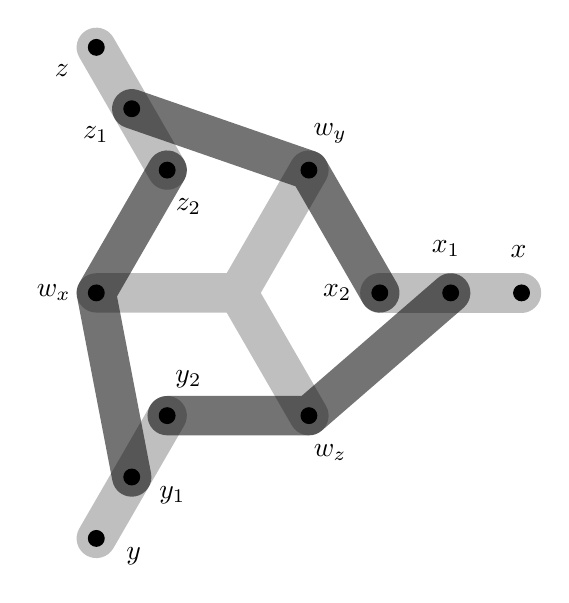
\begin{tikzpicture}[scale=1.8]

\def\rot{0}
\def\dir{-1}
\foreach \x in {1,...,3}{%
  \coordinate (\x-2) at ({\rot+\dir*360/3 * (\x - 1)}:1) {};
  \coordinate (\x-2-l) at ({\rot+\dir*360/3 * (\x - 1)}:0.7) {};
  \coordinate (\x-1) at ({\rot+\dir*360/3 * (\x - 1)}:1.5) {};
  \coordinate (\x-1-l) at ({\rot+\dir*360/3 * (\x - 1-0.1)}:1.5) {};
  \coordinate (\x-0) at ({\rot+\dir*360/3 * (\x - 1)}:2) {};
  \coordinate (\x-0-l) at ({\rot+\dir*360/3 * (\x - 1-0.07)}:2) {};
  \coordinate (\x-w) at ({\rot+\dir*360/3 * (\x + 0.5)}:1) {};
  \coordinate (\x-w-l) at ({\rot+\dir*360/3 * (\x + 0.5)}:1.3) {};
  \node [vertex] at (\x-2) {};
  \node [vertex] at (\x-1) {};
  \node [vertex] at (\x-0) {};
  \node [vertex] at (\x-w) {};
}
\begin{scope}[opacity=0.25, transparency group]
%\fill (1-w) circle (1.37mm);
%\fill (2-w) circle (1.37mm);
%\fill (3-w) circle (1.37mm);
%\fill (0,0) circle (1.37mm);
\draw[line width=5mm,line join=round,line cap=round] (1-w) -- (0,0) -- (2-w);
\draw[line width=5mm,line join=round,line cap=round] (3-w) -- (0,0);
\end{scope}

\node at (1-2-l) {$x_2$};
\node at (2-2-l) {$y_2$};
\node at (3-2-l) {$z_2$};
\node at (1-1-l) {$x_1$};
\node at (2-1-l) {$y_1$};
\node at (3-1-l) {$z_1$};
\node at (1-0-l) {$x$};
\node at (2-0-l) {$y$};
\node at (3-0-l) {$z$};
\node at (1-w-l) {$w_x$};
\node at (2-w-l) {$w_y$};
\node at (3-w-l) {$w_z$};

\draw[draw opacity=0.55,line width=5mm,line cap=round,line join=round] (2-1) -- (1-w) -- (3-2);
\draw[draw opacity=0.55,line width=5mm,line cap=round,line join=round] (3-1) -- (2-w) -- (1-2);
\draw[draw opacity=0.55,line width=5mm,line cap=round,line join=round] (1-1) -- (3-w) -- (2-2);
\draw[draw opacity=0.25,line width=5mm,line cap=round,line join=round] (1-0) -- (1-1) -- (1-2);
\draw[draw opacity=0.25,line width=5mm,line cap=round,line join=round] (2-0) -- (2-1) -- (2-2);
\draw[draw opacity=0.25,line width=5mm,line cap=round,line join=round] (3-0) -- (3-1) -- (3-2);

\end{tikzpicture}
\end{center}

\caption{\label{fig:absorber}An illustration of an absorber for $\left(x,y,z\right)$.
The light edges are the covering matching and the dark edges are the
non-covering matching.}
\end{figure}

Now we explain how absorbers are put together. The relative positions
of the absorbers will be determined by a ``template'' structure,
as follows.
\begin{lem}
\label{lem:resilient-template}For any sufficiently large $n$, there
exists a 3-uniform hypergraph $T$ with $10n$ vertices, at most $160n$
hyperedges and a ``flexible set'' $Z$ of $2n$ vertices, such that
if we remove any $n$ vertices from $Z$, the resulting hypergraph
has a perfect matching. We call this $H$ a \emph{resilient template}.
\end{lem}
To prove \ref{lem:resilient-template} we use the following lemma
of Montgomery \cite[Lemma~2.8]{Mon14}
\begin{lem}
\label{lem:montgomery}For any sufficiently large $n$, there exists
a bipartite graph $H$ on vertex classes $X$ and $Y\sqcup Z$ with
$\left|X\right|=3n$, $\left|Y\right|=\left|Z\right|=2n$, and maximum
degree 40, such that if we remove any $n$ vertices from $Z$, the
resulting bipartite graph has a perfect matching.
\end{lem}
\begin{proof}[Proof of \ref{lem:resilient-template}]
Consider the bipartite graph $H$ from \ref{lem:montgomery} on the
vertex set $X\sqcup Y\sqcup Z$. Add a set $W$ of $\left|X\right|$
new vertices and put a perfect matching between $W$ and $X$, to
obtain a $10n$-vertex tripartite graph $H'$. Now, define our resilient
template with flexible set $Z$ by putting a hyperedge with the vertices
of each of the (at most $160n$) paths of length 2 in $H'$.
\end{proof}
Now we can describe our absorbing structure in its entirety.
\begin{defn}
An \emph{absorbing structure} is a 3-uniform hypergraph of the following
form. Consider a resilient template and put externally vertex-disjoint
absorbers on each edge of the template, introducing 9 new vertices
for each. (Note that the template just describes the relative positions
of the absorbers, its edges are not actually in the absorbing structure).
\end{defn}
Note that an absorbing structure with a flexible set of size $n$
has $10n+9\times160n=O\left(n\right)$ vertices and at most $7\times160n=O\left(n\right)$
edges. Now, we show how absorbers can be used to find perfect matchings.
\begin{lem}
\label{lem:PM-via-absorbers}Consider a 3-uniform hypergraph $S$
(with vertex set $V$, $\left|V\right|=n$) satisfying the following
properties for some $\delta=\delta\left(n\right)=o\left(1\right)$
and fixed $\beta>0$.
\begin{enumerate}
\item There is an absorbing structure $H$ in $S$ with at most $\delta n$
vertices and a flexible set $Z$ of size $\delta^{2}n$.
\item For at most $\delta n$ of the vertices $v\in V$, we have $\left|\left\{ \left\{ x,y\right\} \subseteq Z:\left\{ v,x,y\right\} \in S\right\} \right|<2\delta^{3}n$.
That is to say, few vertices have low degree into the flexible set
$Z$, in $S$.
\item Every vertex subset $W\subseteq V$ with $\left|W\right|\ge\delta^{3}n$
induces at least $\left(1-\beta\right)\left|W\right|^{3}/\left(6n\right)$
hyperedges
\end{enumerate}
Then $S$ has 
\[
\left(\frac{n}{2e^{2}}\left(1-\beta-O\left(\delta\log n\right)\right)\right)^{n/3}
\]
perfect matchings.
\end{lem}
\begin{proof}
We can assume $\delta<1/4$, so that we can greedily choose a $\delta n$-vertex
matching in $V\backslash V'$ containing each of the vertices violating
the second condition. There are $n'=n-v\left(H\right)-\delta n\ge\left(1-2\delta\right)n$
vertices in $V\backslash V\left(H\right)$ remaining unmatched.

Next, repeatedly choose an edge in the remaining unmatched vertices
in $V\backslash V\left(H\right)$ until there are only $\delta^{3}n$
such vertices remaining unmatched. (This means we take a matching
with $m=\left(n'-\delta^{2}n\right)/3=n/3-O\left(\delta n\right)$
edges). The number of ways to make this ordered sequence of choices
is at least
\begin{align}
\prod_{i=1}^{m}\left(1-\beta\right)\frac{\left(n'-3i\right)^{3}}{6n} & =\left(\frac{1-\beta}{6n}\right)^{m}\exp\left(\sum_{i=1}^{m}\log\left(n'-3i\right)^{3}\right)\label{eq:num-matchings}\\
 & =\left(\frac{\left(1-\beta\right)\left(n'\right)^{3}}{6n}\right)^{m}\exp\left(n'\sum_{i=1}^{m}\frac{3}{n'}\log\left(1-3\frac{i}{n'}\right)\right).\nonumber 
\end{align}
Since $\log\left(1-3t\right)$ is a decreasing function of $t$, we
have
\[
\sum_{i=1}^{m}\frac{1}{n'}\log\left(1-3\frac{i}{n'}\right)\le\int_{0}^{m/n'}3\log\left(1-3t\right)\d t\le\sum_{i=1}^{n'/3}\frac{1}{n'}\log\left(1-3\frac{i-1}{n'}\right).
\]
Noting that
\begin{align*}
\sum_{i=1}^{m}\left(\log\left(1-3\frac{i-1}{n'}\right)-\log\left(1-3\frac{i}{n'}\right)\right) & =\sum_{i=1}^{m}\left(\log\left(1+\frac{3}{n'-3i}\right)\right)\\
 & \le3\sum_{i=1}^{m}\frac{1}{n'-3i}=O\left(\log n\right)
\end{align*}
and that $\int\log s\d s=s\left(\log s-1\right)$, we have
\begin{align*}
\sum_{i=1}^{n'/3}\frac{3}{n'}\log\left(1-3\frac{i}{n'}\right) & =\int_{0}^{1/3-O\left(\delta\right)}3\log\left(1-3t\right)\d t+O\left(\frac{\log n}{n}\right)\\
 & =\int_{O\left(\delta\right)}^{1}\log s\d s+O\left(\frac{\log n}{n}\right)\\
 & =-1-O\left(\delta\log\left(n\right)\right).
\end{align*}
So, the expression in \ref{eq:num-matchings} is equal to
\begin{align*}
\left(\left(1-\beta\right)\frac{n^{2}}{6}\right)^{n'/3}e^{-n}n^{O\left(\delta n\right)} & =\left(\frac{n^{2}}{6e^{3}}\right)^{n/3}n^{O\left(\delta n\right)}.
\end{align*}
Dividing by $m!=\left(n/\left(3e\right)\right)^{n/3}n^{O\left(\delta n\right)}$
(because we were counting ordered matchings), there are at least$\left(n/\left(2e^{2}\right)\right)^{n/3}n^{O\left(\delta n\right)}$
ways to choose a matching in $V\backslash V\left(H\right)$ covering
all but $\delta^{3}n$ vertices, none of which violate the second
condition. We can greedily extend such a matching to cover half of
$Z$ using the second and third conditions. By the defining property
of a resilient template, there is a perfect matching in the subgraph
of the template induced by the vertices uncovered so far. For each
hyperedge of this perfect matching, use the covering matching of the
corresponding absorber; for each other hyperedge in the template use
the non-covering matching.
\end{proof}

\subsection{Absorbing properties in the triangle removal process\label{sec:absorbers-in-TRP}}

In this section we prove that the properties in \ref{lem:PM-via-absorbers}
(for say $\delta=1/\log^{2}n$ and arbitrarily small $\beta$) hold
in the triangle removal process, conditioned on a certain quasirandomess
event, with probability $1-\exp\left(-\tilde{\Omega}\left(n^{2}\right)\right)$.
(A tilde above asymptotic nation indicates that polylogarithmic factors
are being ignored). This will allow us to use \ref{lem:triangle-removal-transfer}
to deduce that the same is true for a uniformly random Steiner triple
system, proving \ref{thm:PM-in-STS}.

Fix a large constant $h\in\NN$ (we will see later exactly how large
it should be), and consider arbitrarily small $\alpha>0$. We will
treat $\alpha$ as a constant, but asymptotics in this section will
be mostly uniform over $\alpha$.

\subsubsection{\label{subsec:absorbers}Absorbers}

First we find absorbers. Note that $K_{n}$ is $\left(n^{1/2},h\right)$-quasirandom,
and let $a=a\,b\left(1/2,h\right)$ in the notation of \ref{lem:triangle-removal-analysis},
so that $\cordm{n^{-a},h}{\alpha N}$ is nonempty. Let $b=b\left(a\right)$
in the notation of \ref{lem:bite-transfer}. As in \ref{lem:bite-transfer},
let $\mathcal{Q}=\left\{ S\in\cordm{n^{-b},h}{2\alpha N}:S_{\alpha N}\in\cordm{n^{-a},h}{\alpha N}\right\} \supseteq\cordm{n^{-a},h}{2\alpha N}$.
Let $\randS\in\rg n{2\alpha n}$, conditioned on the event $\randS\in\mathcal{Q}$,
and condition on any $\randS_{\alpha N}=S\in\cordm{n^{-a},h}{\alpha N}$.
We will use \ref{lem:bite-transfer} to analyse $\randS\backslash\randS_{\alpha N}\in\rg S{\alpha N}$
via $\GSnp S{\alpha/N}$. So, let $\randS^{*}\in\GSnp S{\alpha/N}$
be obtained from $\randG\in\Gnp S{\alpha/N}$.

By quasirandomness, every vertex has degree $\left(1\pm n^{-a}\right)\left(1-\alpha\right)n$
$\left(1\pm n^{-a}\right)\alpha n/2=\Omega\left(\alpha n\right)$
in $S$. Consider vertices $x,y,z$. Say an \emph{absorber-extension}
is a collection of 4 hyperedges which forms an absorber on $x,y,z$
when combined with three edges of $S$ incident to $x,y,z$. Let $\randY$
be the maximum size of an edge-disjoint collection of absorber-extensions
in $\randS^{*}$. That is, it is the maximal size of a collection
of hyperedge-disjoint isolated absorber-extensions in $\randG$, where
we say a subgraph of $\randG$ is \emph{isolated} if none of its hyperedges
intersect another hyperedge of $\randG$ in more than one vertex.
Now, adding a hyperedge to a hypergraph can invalidate at most three
absorber-extensions in a maximal collection, and removing a hyperedge
can remove at most one absorber-extension in a maximal collection.
So, changing the presence of one edge of $\randG$ can change $\randY$
by at most 3. By \ref{thm:bernstein-type},
\begin{equation}
\Pr\left(\randY\le\E\randY-t\right)\le\exp\left(-\Omega\left(\frac{t^{2}}{3^{2}{n \choose 3}\alpha/n+3t}\right)\right)=\exp\left(-\Omega\left(\frac{t^{2}}{\alpha n^{2}+t}\right)\right).\label{eq:disjoint-absorber-bite-tail}
\end{equation}

Let $\randX$ be the number of isolated absorber-extensions in $\randG$
and let $\randZ$ be the number of pairs of hyperedge-intersecting
absorber-extensions in $\randG$. We can obtain a collection of disjoint
isolated absorber-extensions by considering the collection of all
isolated absorber-extensions and deleting one from each intersecting
pair, so $\randY\ge\randX-\randZ$ and $\E\randY\ge\E\randX-\E\randZ$.

If $h$ is large enough and $\alpha$ is small enough, there are $\Theta\left(\alpha^{3}n^{6}\right)$
possible absorber-extensions not conflicting with $S$. Indeed, to
choose such a candidate absorber-extension, first choose three hyperedges
$e_{x},e_{y},e_{z}$ incident to $x,y,z$ (there are $\left(\alpha n\right)^{3}$
ways to do this). Then, consider the graph $H$ obtained by removing
the three rooted hyperedges of an absorber and replacing the remaining
hyperedges with triangles. The number of ways to complete our candidate
absorber-extension is precisely the number of copies of $H$ rooted
on the vertices of $e_{x},e_{y},e_{z}$ in the obvious way, in $G\left(S\right)$.
By \ref{lem:H-count} this number is $\left(1-\alpha\right)^{O\left(1\right)}n^{3}=\Theta\left(n^{3}\right)$.
The probability each possible absorber-extension occurs and is isolated
in $\randG$ is $\Theta\left(\left(\alpha/n\right)^{4}\left(1-\alpha/n\right)^{O\left(n\right)}\right)=\Theta\left(\alpha^{4}n^{-4}\right)$.
So, $\E\randX=\Theta\left(\alpha^{7}n^{2}\right)$.

Now, there are several possibilities for a hyperedge-intersecting
pair of distinct absorber-extensions.
\begin{itemize}
\item they could intersect in the unrooted hyperedge of the covering matching
of the absorber. There are $\Theta\left(\left(\alpha n\right)^{6}n^{3}\right)$
possibilities for such a pair of absorber-extensions, and each occurs
with probability $\Theta\left(\left(\alpha/n\right)^{7}\right)$,
so the expected number of such is $\Theta\left(\alpha^{13}n^{2}\right)$.
\item They could intersect in the unrooted hyperedge of the covering matching
as above, and also in one hyperedge of the non-covering matching''.
There are $\Theta\left(\left(\alpha n\right)^{4}n^{3}\right)$ possible
such pairs, and each occurs with probability $\Theta\left(\left(\alpha/n\right)^{6}\right)$,
so the expected number of such is $\Theta\left(\alpha^{10}n\right)$.
\item They could intersect in one edge of the non-covering matching. There
are $\Theta\left(\left(\alpha n\right)^{4}n^{5}\right)$ possible
such pairs, and each occurs with probability $\Theta\left(\left(\alpha/n\right)^{7}\right)$,
so the expected number of such is $\Theta\left(\alpha^{11}n^{2}\right)$.
\item They could intersect in two edges of the non-covering matching. There
are $\Theta\left(\left(\alpha n\right)^{3}n^{4}\right)$ possible
such pairs, and each occurs with probability $\Theta\left(\left(\alpha/n\right)^{6}\right)$,
so the expected number of such is $\Theta\left(\alpha^{9}n\right)$.
\end{itemize}
In summary (for small $\alpha$), we have $\E\randZ=O\left(\alpha^{11}n^{2}\right)$,
so $\E\randY=\Theta\left(\alpha^{7}n^{2}\right)$. Considering $\alpha$
as fixed, \ref{eq:disjoint-absorber-bite-tail} gives $\randY=\Omega\left(n^{2}\right)$
with probability $1-\exp\left(-\Omega\left(n^{2}\right)\right)$.

Note that if there are $\Omega\left(n^{2}\right)$ edge-disjoint absorber-extensions
then there must in fact be $\Omega\left(n\right)$ vertex-disjoint
absorber-extensions. We can find these greedily; the degree in $\randS$
of each vertex is $O\left(n\right)$, so deleting $O\left(1\right)$
vertices can delete at most $O\left(n\right)$ edges. By the union
bound and \ref{lem:bite-transfer}, it follows that with probability
$1-\exp\left(-\Omega\left(n^{2}\right)\right)$, every triple of vertices
has $\Omega\left(n\right)$ externally vertex-disjoint absorbers in
$\randS$.

If $\randS$ has this property, then we can greedily build our absorbing
structure, as follows. Recalling that $\delta=o\left(1\right)$, choose
a resilient template $H$ with $O\left(\delta^{2}n\right)$ hyperedges,
on $O\left(\delta^{2}n\right)$ vertices of $\randS$, such that the
flexible set is $Z=\range{\delta^{2}n}$ for some fixed $c>0$. Noting
that an absorber has $O\left(1\right)$ non-rooted vertices, we can
greedily find an absorber in $\randS$ on each edge of $H$, in an
externally vertex-disjoint fashion. The entire absorbing structure
then has $O\left(\delta^{2}n\right)\le\delta n$ vertices. This proves
that the first property of \ref{lem:PM-via-absorbers} holds with
probability $1-\exp\left(-\Omega\left(n^{2}\right)\right)$ in $\randS$
(conditioned on $\mathcal{Q}$), and by \ref{lem:triangle-removal-transfer}
it therefore holds a.a.s. in a uniformly random Steiner triple system.
(Actually, what we have proved is slightly stronger, because we can
specify the location of the flexible set of the absorbing structure).

\subsubsection{High degree into the flexible set}

Recall that $\delta=1/\log^{2}n=\tilde{\Theta}\left(1\right)$. With
$\randS^{*}\in\GSnp n{\alpha/N}$ obtained from $\randG\in\Gnp n{\alpha/N}$,
fix a set $W$ with $\delta n$ vertices and let $\randY$ be the
number of edges of $\randS^{*}$ with one vertex in $W$ and two vertices
in the set $Z=\range{\delta^{2}n}$. That is, $\randY$ the number
of such edges in $\randG$ that are ``isolated''. There are $\Theta\left(\left(\delta n\right)^{2}n\right)=\Theta\left(n^{3}\log^{-O\left(1\right)}n\right)$
possible edges and each is present and isolated with probability $\left(\alpha/n\right)\left(1-\alpha/n\right)^{O\left(n\right)}=\Theta\left(n^{-1}\right)$,
so $\E\randY=\tilde{\Theta}\left(n^{2}\right)$ and just as in the
preceding argument, \ref{thm:bernstein-type} shows that for some
$\delta$, with probability $1-\exp\left(-\tilde{\Omega}\left(n^{2}\right)\right)$
we have $\randY\ge2\delta^{3}n^{2}/4$. This is not possible unless
there is a vertex $v$ in $W$ with degree $2\delta^{3}n$ in $Z$,
in $\randS^{*}$. Since there are fewer than $2^{n}=e^{o\left(n^{2}\right)}$
choices for $W$, the union bound and \ref{lem:bite-transfer} prove
that with probability $1-\exp\left(-\tilde{\Omega}\left(n^{2}\right)\right)$
every set $W$ has such a vertex (and therefore the second condition
of \ref{lem:PM-via-absorbers} holds), in an instance of the triangle
removal process $\rg n{\alpha N}$. Applying \ref{lem:triangle-removal-transfer}
with $S=\varnothing$ proves that the same holds a.a.s. in a uniformly
random Steiner triple system.

\subsubsection{Density in subsets\label{subsec:density}}

Fix a set $W\subseteq V$ with $\left|W\right|\ge\delta^{3}n$. With
$\randS^{*}$ and $\randG$ as in the previous subsection, redefine
$\randY$ to be the number of edges of $\randS^{*}$ included in $W$.
There are $\left(1+o\left(1\right)\right)\left|W\right|^{3}/6$ possible
edges, and each is present and isolated in $\randG$ with probability
$\left(\alpha/n\right)\left(1-\alpha/n\right)^{O\left(n\right)}=\left(\alpha/n\right)\left(1-O\left(\alpha\right)\right)$,
so with the same reasoning as in the previous two sections, \ref{thm:bernstein-type}
shows that with probability $1-\exp\left(-\tilde{\Omega}\left(n^{2}\right)\right)$
we have $\randY\ge\alpha\left(1-O\left(\alpha\right)\right)\left|W\right|^{3}/\left(6n\right)$.
The union bound and \ref{lem:bite-transfer} proves that this holds
for any $W$ with probability $1-\exp\left(-\tilde{\Omega}\left(n^{2}\right)\right)$,
in an instance of the triangle removal process $\rg n{\alpha N}$.
Therefore by \ref{lem:triangle-removal-transfer} it holds a.a.s.
in $\randS_{\alpha N}$ for a uniformly random $\randS\in\S$. By
symmetry, this property also holds a.a.s. in $\randS_{k\alpha N}\backslash\randS_{\left(k-1\right)\alpha N}$
for any $k\le1/\alpha$ (we impose that $1/\alpha$ is an integer).
So the total number of edges in $\randS$ induced by any $W$ is $\left(1-O\left(\alpha\right)\right)\left|W\right|^{3}/\left(6n\right)$.
For $\beta$ a large multiple of $\alpha$, the third condition in
\ref{lem:PM-via-absorbers} is then satisfied.

\section{An upper bound for the number of perfect matchings\label{sec:max-num-matchings}}

\global\long\def\randl{\boldsymbol{\lambda}}

\global\long\def\randz{\boldsymbol{z}}

\global\long\def\randR{\boldsymbol{R}}

\global\long\def\rande{\boldsymbol{e}}

\global\long\def\randQ{\boldsymbol{Q}}

In this section we prove \ref{thm:maximum-PMs}, with the entropy
method. See \cite{LL13} for a brief introduction to the notion of
entropy as necessary for proving upper bounds of this type.
\begin{proof}
Let $\mathcal{M}$ be the set of perfect matchings in $S$. Consider
a uniformly random $\randM\in\mathcal{M}$ and let $H\left(\randM\right)=\log\left|\mathcal{M}\right|$
be the entropy of $\randM$. Let $\randM_{v}$ be the hyperedge of
$\randM$ containing the vertex $v$, so that the sequence $\left(\randM_{v}\right)_{v\in\range n}$
determines $\randM$. For any ordering on the vertices of $S$,
\[
H\left(M\right)=\sum_{v\in V}H\left(\randM_{v}\cond\randM_{v'}:v'<v\right).
\]
Now, a sequence $\lambda\in\left[0,1\right]^{n}$ with all $\lambda_{v}$
distinct induces an ordering on $\range n$, with $v'<v$ when $\lambda_{v'}>\lambda_{v}$.
Let $\randR_{v}\left(\lambda\right)$ be 1 plus the number of 3-edges
$e\ne\randM_{v}$ such that $\lambda_{v'}<\lambda_{v}$ for all $v'\in\bigcup_{x\in X}\randM_{x}$.
(So, $\randR_{v}\left(\lambda\right)=1$ if $\lambda_{v'}>\lambda_{v}$
for some $v'\in\randM_{v}\backslash\left\{ v\right\} $). This is
an upper bound on the number of possible values for $\randM_{v}$
given the information  $\left(\randM_{v'}\,\colon\,\lambda_{v'}>\lambda_{v}\right)$.
Let
\[
R_{v}^{M,\lambda}=\E\left[\randR_{v}\left(\randl\right)\cond\randM=M,\,\randl_{v}=\lambda,\,\lambda_{v'}<\lambda_{v}\text{ for all }v'\in\randM_{v}\backslash\left\{ v\right\} \right].
\]
(Note that $\randl_{v}=\lambda$ occurs with probability zero, so
formally we should condition on $\randl_{e}=\lambda\pm\d\lambda$
and take limits in what follows, but there are no continuity issues
so we will ignore this detail). By linearity of expectation, we have
\[
R_{v}^{M,\lambda}=\left(\left(n-1\right)/2-1\right)\lambda^{6},
\]
because there are $\left(n-1\right)/2$ edges in $S$ containing $v$,
and for each such edge $e$ other than $\randM_{v}$ the two non-$v$
vertices must be matched to different 3-edges in $\randM$ (if they
were matched to the same edge that edge would intersect $e$ in two
vertices, violating the defining property of a Steiner triple system).
By Jensen's inequality,
\[
\E\left[\log\randR_{v}\left(\randl\right)\cond\randM=M,\,\randl_{v}=\lambda,\,\lambda_{v'}<\lambda_{v}\text{ for all }v'\in\randM_{v}\backslash\left\{ v\right\} \right]\le\log R_{v}^{M,\lambda},
\]
and
\[
\Pr\left(\lambda_{v'}<\lambda_{v}\text{ for all }v'\in\randM_{v}\backslash\left\{ v\right\} \right)=\lambda^{2}
\]
so
\[
\E\left[\log\randR_{v}\left(\randl\right)\cond\randM=M,\,\randl_{v}=\lambda\right]\le\lambda^{2}\log R_{v}^{M,\lambda}.
\]
For any $M\in\mathcal{M}$ we then have
\begin{align*}
\E\left[\log\randR_{v}\left(\randl\right)\cond\randM=M\right] & \le\E\left[\randl_{v}^{2}\log R_{v}^{M,\randl_{i}}\right]\\
 & =\int_{0}^{1}\lambda^{2}\log\left(\left(\left(n-1\right)/2-1\right)\lambda^{6}\right)\d\lambda\\
 & =\frac{1}{3}\left(\log\left(\left(1+o\left(1\right)\right)n/2\right)-2\right),
\end{align*}
using the fact that $\int_{0}^{1}\lambda^{A-1}\log\left(C\lambda^{B}\right)\d t=A^{-1}\log C-A^{-2}B$
for any $A,B,C>0$. We conclude that
\begin{align*}
\log\left|\mathcal{M}\right| & \le H\left(\randM\right)\\
 & \le\sum_{i\in\range n}\E\left[\log\randR_{i}\left(\randl\right)\right]\\
 & \le\frac{n}{3}\left(\log\left(\left(1+o\left(1\right)\right)n/2\right)-2\right)
\end{align*}
which is equivalent to the theorem statement.
\end{proof}

\section{Latin squares\label{sec:latin}}

In this section we briefly sketch how one should adapt the methods
in this paper to prove \ref{thm:latin}.

The main difference from the case of Steiner triple systems is that
instead of considering triangles in graphs (subgraphs of $K_{n}$),
we consider triangles in subgraphs of the complete tripartite graph
$K_{n,n,n}$. In this section we use the notation $V=V_{1}\sqcup V_{2}\sqcup V_{3}$
for the vertex partition of $K_{n,n,n}$. We say a subgraph $G\subseteq K_{n,n,n}$
with $m$ edges between each pair of parts is $\left(\varepsilon,h\right)$-quasirandom
if for each $i\in\left\{ 1,2,3\right\} $, every set $A\subseteq V\backslash V_{i}$
with $\left|A\right|\le h$ has $\left(1\pm\varepsilon\right)\left(m/n^{2}\right)^{\left|A\right|}n$
common neighbours in $V_{i}$. We believe that the following result
should follow from a slight adaptation of the proof in \cite{Kee15}.
\begin{conjecture}
There are $h\in\NN$, $\varepsilon_{0},a\in\left(0,1\right)$ and
$n_{0},\ell\in\NN$ such that if $n\ge n_{0}$, $m/n^{2}\ge n^{-a}$
and $\varepsilon\le\varepsilon_{0}\left(m/n^{2}\right){}^{\ell}$,
and $G\subseteq K_{n,n,n}$ is $\left(\varepsilon,h\right)$-quasirandom
with $m$ edges between each pair of parts, then the edges of $G$
can be decomposed into triangles.
\end{conjecture}
Redefining $\ord$, $\ordm m$ and $\cordm{\varepsilon,h}m$ in the
obvious way for ordered (partial) Latin squares and redefining $\RR\left(n,m\right)$
to be the distribution on $\ordm m$ obtained with $m$ steps of the
triangle removal process starting from $K_{n,n,n}$, we can then prove
a counterpart to \ref{lem:triangle-removal-transfer} for random Latin
squares, with virtually the same proof.
\begin{sol}
\label{thm:latin-transfer}There is $h_{0}\in\NN$ such that for fixed
$h\ge h_{0}$ and sufficiently small $a$ there is $b\left(a\right)>0$
such that the following holds. Fix $\alpha\in\left(0,1\right)$, let
$\mathcal{P}\subseteq\ordm{\alpha N}$ be a property of ordered partial
Latin squares, let $\mathcal{Q}\supseteq\cordm{n^{-a},h}{\alpha N}$,
let $\randS\in\ord$ be uniformly random and let $\randS'\in\rg n{\alpha N}$.
If
\[
\Pr\left(\randS'\notin\mathcal{P}\cond\randS'\in\mathcal{Q}\right)<\exp\left(-n^{2-b}\right)
\]
then
\[
\Pr\left(\randS_{\alpha N}\notin\mathcal{P}\right)=\exp\left(-\Omega\left(n^{1-2a}\right)\right).
\]
\end{sol}
Now we outline what should be adapted from the arguments in \ref{sec:absorbers}
for the Latin squares case. The definition of an absorber can remain
the same, noting that the hypergraph in \ref{def:absorber} is tripartite
(if $x,y,z$ are in different parts, then an absorber on $\left(x,y,z\right)$
can be chosen with each 3-edge having a vertex in each part). The
definition of a resilient template should be adapted slightly: a resilient
template is a tripartite hypergraph $H$ with a flexible set $Z$
satisfying $\left|Z\cap V_{1}\right|=\left|Z\cap V_{2}\right|=\left|Z\cap V_{3}\right|$,
such that if half the vertices are removed from each $Z\cap V_{i}$
the remaining hypergraph has a perfect matching. To prove a counterpart
of \ref{lem:resilient-template} we can just use three copies (one
for each $V_{i}$) of the construction in the proof of \ref{lem:resilient-template}.
The counterpart of \ref{lem:PM-via-absorbers} is as follows (with
virtually the same proof).
\begin{lem}
\label{lem:absorbers-latin}Consider a 3-uniform tripartite hypergraph
$L\subseteq K_{n,n,n}^{\left(3\right)}$ satisfying the following
properties for some $\delta=\delta\left(n\right)=o\left(1\right)$
and fixed $\beta>0$.
\begin{enumerate}
\item There is an absorbing structure $H$ in $L$ with at most $\delta n$
vertices and a flexible set $Z$ intersecting each $V_{i}$ in $\delta^{2}n$
vertices.
\item For at most $\delta n$ of the vertices $v\in V_{1}$, we have $\left|\left\{ \left(x,y\right)\in V_{2}\times V_{3}:\left(v,x,y\right)\in L\right\} \right|<3\delta^{3}n$,
and similarly most $v\in V_{2}$ and $v\in V_{3}$ have high degree
into $V_{1}\times V_{3}$ and $V_{1}\times V_{2}$ respectively.
\item For any choice of $W_{i}\subseteq V_{i}$ such that each $\left|W_{i}\right|\ge\delta^{3}n$,
there are at least $\left(1-\beta\right)\left|W_{1}\right|\left|W_{2}\right|\left|W_{3}\right|/n$
hyperedges in $W_{1}\times W_{2}\times W_{3}$.
\end{enumerate}
Then $L$ has 
\[
\left(\frac{n}{e^{2}}\left(1-\beta-O\left(\delta\log n\right)\right)\right)^{n}
\]
transversals.
\end{lem}
One can then use \ref{lem:absorbers-latin} and \ref{thm:latin-transfer}
to prove \ref{thm:latin} in basically the same way as the proof of
\ref{thm:PM-in-STS} in \ref{sec:absorbers-in-TRP}.

\section{Concluding remarks\label{sec:concluding}}

In this paper we introduced a new method for analysing random Steiner
triple systems, and we used it to prove that almost all Steiner triple
systems have many perfect matchings. There are many interesting open
questions that remain.
\begin{itemize}
\item We believe the most interesting problem that seems approachable by
our methods is to prove that almost all Steiner triple systems (and
Latin squares) can be decomposed, or at least approximately decomposed,
into disjoint perfect matchings (transversals). The proof of \ref{thm:PM-in-STS}
can be easily modified to prove that almost all Steiner triple systems
have $\Omega\left(n\right)$ disjoint perfect matchings, but to find
$\left(1-o\left(1\right)\right)n/2$ disjoint perfect matchings would
require a new idea. For Latin squares, the property of being decomposable
into transversals is equivalent to the important property of having
an \emph{orthogonal mate}, which has a long history dating back to
Euler. More details can be found in \cite{Wan11}.
\item A $\left(q,r\right)$-Steiner system ($q>r$) is a $q$-uniform hypergraph
such that every $r$-set of vertices is included in exactly one hyperedge
(so, a Steiner triple system is a $\left(3,2\right)$-Steiner system).
We believe that our results should generalize to Steiner systems with
any combination of parameters, and the main difficulty probably lies
in coming up with a suitable absorber. Note that a perfect matching
is actually a $\left(q,1\right)$-Steiner system, so if $r>2$ then
there is the more general (and much more difficult) question of whether
$\left(q,r\right)$-Steiner systems typically contain $\left(q,r'\right)$-Steiner
systems, for all $r'<r$. It might even be true that almost all $\left(q,r\right)$-Steiner
systems can be ``completely decomposed'' in the sense that they
can be partitioned into disjoint $\left(q,r-1\right)$-Steiner systems,
which can be partitioned into $\left(q,r-2\right)$-Steiner systems,
and so on. A similar phenomenon occurs for regular subgraphs of random
regular graphs (see \cite[Section~9.5]{JLR00}).
\item Another interesting question about random Steiner triple systems is
whether they contain Steiner triple subsystems on fewer vertices.
McKay and Wanless \cite{MW99} proved that almost all Latin squares
have many small Latin subsquares, but it was conjectured by Quackenbush
\cite{Qua80} that most Steiner triple systems do not have proper
subsystems. It seems unlikely that the methods in this paper will
be able to prove or disprove this conjecture without substantial new
ideas; actually by consideration of the random 3-graph $\Gnp n{1/n}$
we suspect the expected number of 7-vertex Steiner triple systems
(Fano planes) in a random Steiner triple system is $\Theta\left(1\right)$,
and that the distribution of this number is asymptotically Poisson.
\item We could ask more generally about containment and enumeration of subgraphs.
Is it true that every fixed hypergraph $H$ whose every subgraph has
more vertices than edges, appears a.a.s. in a random Steiner triple
system? Can we show that moreover the number of copies of $H$ is
concentrated? The methods in this paper can probably be used to prove
a lower bound for the number of copies of $H$ when every subgraph
of $H$ has at least 2 more vertices than edges, but due to the ``infamous
upper tail'' issue (see \cite{JR02}), an upper bound for the number
of copies of $H$ is likely to be more difficult.
\item One of the most fundamental properties of random graphs and hypergraphs
is that they have low \emph{discrepancy}, meaning that every sufficiently
large subset of vertices has about the expected number of edges. In
\ref{subsec:density} we effectively proved a very weak discrepancy
bound, but it is not clear how to use our methods to reach anywhere
near optimal discrepancy. See \cite{LL15} for some conjectures about
discrepancy of Latin squares and their high-dimensional relatives.
\end{itemize}
\bibliographystyle{amsplain_initials}
\bibliography{references}

\begin{appendices}
\crefalias{section}{appsec}

\section{\label{sec:keevash}Counting completions of Steiner triple systems}

\global\long\def\coG{G}

\global\long\def\Sext#1{\mathcal{S}^{\mathrm{ext}}\left(#1\right)}

\global\long\def\randl{\boldsymbol{\lambda}}

\global\long\def\randz{\boldsymbol{z}}

\global\long\def\randR{\boldsymbol{R}}

In this section we prove \ref{prop:num-extensions}. This is accomplished
with minor adaptations of proofs by Linial and Luria \cite{LL13}
and Keevash \cite{Kee15}. As in \ref{sec:outline}, let $N={n \choose 2}/3$
and assume that $n$ is 1 or 3 mod 6.

For a partial system $S\in\S_{\alpha N}^{n^{-a}}$, let $\Sext S$
be the number of Steiner triple systems that contain $S$. We want
to determine $\left|\ext S\right|=\left(N-\alpha N\right)!\left|\Sext S\right|$
up to a factor of $e^{n^{2-b}}$ (for some $b$).

First, we can get an upper bound via the method of Linial and Luria
\cite{LL13}. The reader should refer to that paper for more detailed
exposition and a brief introduction to the notion of entropy.
\begin{thm}
\label{thm:number-of-completions-upper}For any $a>0$, any $\alpha\in\left[0,1\right]$,
and any $S^{*}\in\cSm{n^{-a},2}{\alpha N}$,
\[
\left|\Sext{S^{*}}\right|\le\left(\left(1+O\left(n^{-a}\right)\right)\left(\frac{1-\alpha}{e}\right)^{2}n\right)^{N\left(1-\alpha\right)}.
\]
\end{thm}
\begin{proof}
Let $\randS\in\Sext{S^{*}}$ be a uniformly random completion of $S$.
Let $H\left(\randS\right)=\log\left|\Sext{S^{*}}\right|$ be the entropy
of $\randS$.

Let $\coG=G\left(S^{*}\right)$. For each $e=\left\{ x,y\right\} \in\coG$,
let $\left\{ x,y,\randz_{e}\right\} $ be the hyperedge that includes
$e$ in $\randS$. So, the sequence $\left(\randz_{e}\right)_{e\in\coG}$
determines $\randS$. For any ordering on the edges of $\coG$, we
have
\[
H\left(\randS\right)=\sum_{e\in\coG}H\left(\randz_{e}\cond\left(\randz_{e'}\,\colon\,e'<e\right)\right).
\]
Now, a sequence $\lambda\in\left[0,1\right]^{E\left(\coG\right)}$
with all $\lambda_{e}$ distinct induces an ordering on the edges
of $\coG$, with $e'<e$ when $\lambda_{e'}>\lambda_{e}$. Let $\randR_{e}\left(\lambda\right)$
be an upper bound on the number of possible values for $\randz_{e}$
given the information $\left(\randz_{e'}\,\colon\,\lambda_{e'}>\lambda_{e}\right)$,
defined as follows. $\randR_{e}=1$ if $\lambda_{\left\{ x,\randz_{e}\right\} }>\lambda_{e}$
or $\lambda_{\left\{ y,\randz_{e}\right\} }>\lambda_{e}$ (because
in this case $\randz_{e}$ is determined), and otherwise $\randR_{e}$
is 1 plus the number of vertices $v\notin\left\{ x,y,\randz_{e}\right\} $
such that $\left\{ x,v\right\} ,\left\{ y,v\right\} \in\coG$ and
$\lambda_{e'}<\lambda_{e}$ for each of the 6 edges $e'\in\coG$ included
in the hyperedges that include $\left\{ x,v\right\} $ and $\left\{ y,v\right\} $
in $\randS$.

Now, note that for any $\lambda$ we have
\[
H\left(\randz_{e}\cond\left(\randz_{e'}\,\colon\,\lambda_{e'}>\lambda_{e'}\right)\right)\le\E\left[\log\randR_{e}\left(\lambda\right)\right].
\]
Let $\randl=\left(\randl_{e}\right)_{e\in\coG}$ be a sequence of
independent random variables, where each $\randl_{e}$ has the uniform
distribution in $\left[0,1\right]$. (Note that almost surely each
$\randl_{e}$ is distinct). By linearity of expectation and the tower
law, 
\[
H\left(\randS\right)=\sum_{e\in\coG}\E\left[\log\randR_{e}\left(\randl\right)\right].
\]
Next, for any $S\in\Sext{S^{*}}$ and $\lambda\in\left[0,1\right]$,
let 
\[
R_{e}^{S,\lambda}=\E\left[\randR_{e}\left(\randl\right)\cond\randS=S,\,\randl_{e}=\lambda,\,\randl_{\left\{ x,\randz_{e}\right\} },\randl_{\left\{ y,\randz_{e}\right\} }<\randl_{e}\right].
\]
Now, in $\coG$, by quasirandomness $x$ and $y$ have $\left(1\pm O\left(n^{-a}\right)\right)\left(1-\alpha\right)^{2}n$
common neighbours. By the discussion above, and linearity of expectation,
we have 
\[
R_{e}^{S,\lambda}=\left(1+O\left(n^{-a}\right)\right)\left(1-\alpha\right)^{2}\lambda^{6}n.
\]
Now, by Jensen's inequality,
\[
\E\left[\log\randR_{e}\left(\randl\right)\cond\randS=S,\,\randl_{e}=\lambda,\,\randl_{\left\{ x,\randz_{e}\right\} },\randl_{\left\{ y,\randz_{e}\right\} }<\randl_{e}\right]\le\log R_{e}^{S,\lambda},
\]
and 
\[
\Pr\left(\randl_{\left\{ x,\randz_{e}\right\} },\randl_{\left\{ y,\randz_{e}\right\} }<\randl_{e}\cond\randl_{e}=\lambda\right)=\lambda^{2},
\]
so
\[
\E\left[\log\randR_{e}\left(\randl\right)\cond\randS=S,\,\randl_{e}=\lambda\right]\le\lambda^{2}\log R_{e}^{S,\lambda}+\left(1-\lambda^{2}\right)\log1=\lambda^{2}\log R_{e}^{S,\lambda}.
\]
For any $S\in\Sext{S^{*}}$, we then have 
\begin{align*}
\E\left[\log\randR_{e}\left(\randl\right)\cond\randS=S\right] & \le\E\left[\lambda^{2}\log R_{e}^{S,\randl_{e}}\right]\\
 & =\int_{0}^{1}\lambda^{2}\log\left(\left(1+O\left(n^{-a}\right)\right)\left(1-\alpha\right)^{2}\lambda^{6}n\right)\d\lambda\\
 & =\frac{1}{3}\left(\log\left(\left(1+O\left(n^{-a}\right)\right)\left(1-\alpha\right)^{2}n\right)-2\right)
\end{align*}
using the fact that $\int_{0}^{1}\lambda^{A-1}\log\left(C\lambda^{B}\right)\d t=A^{-1}\log C-A^{-2}B$
for any $A,B,C>0$. We conclude 
\begin{align*}
\log\left|\Sext{S^{*}}\right| & \le H\left(\randS\right)\\
 & \le\sum_{e\in\coG}\E\left[\log\randR_{e}\left(\randl\right)\right]\\
 & \le\left(N-\alpha N\right)\frac{1}{3}\left(\log\left(\left(1\pm O\left(n^{-a}\right)\right)\left(1-\alpha\right)^{2}n\right)-2\right),
\end{align*}
which is equivalent to the theorem statement.
\end{proof}
For the lower bound, we will count ordered Steiner triple systems.
\begin{thm}
\label{thm:number-of-completions-lower}There is $h\in\NN$ such that
for any $a>0$, there is $b=b\left(a\right)$ such that the following
holds. For any $\alpha\in\left(0,1\right)$ and any $S^{*}\in\cordm{n^{-a},h}{\alpha N}$,
\[
\left|\ext{S^{*}}\right|\le\left|\Sext{S^{*}}\right|\le\left(\left(1+O\left(n^{-b}\right)\right)\left(\frac{1-\alpha}{e}\right)^{2}n\right)^{N\left(1-\alpha\right)}\left(N-\alpha N\right)!.
\]
\end{thm}
To prove \ref{thm:number-of-completions-lower} we will need an analysis
of the triangle removal process (see \ref{sec:Random-triangle-removal})
and the following immediate consequence of \cite[Theorem~2.1]{Kee15}.
\begin{thm}
\label{thm:keevash}There are $h\in\NN$, $\varepsilon_{0},a\in\left(0,1\right)$
and $n_{0},\ell\in\NN$ such that if $S\in\cSm{\varepsilon,h}m$ is
a partial system with $n\ge n_{0}$, with $d\left(G\left(S\right)\right)=1-m/N\ge n^{-a}$
and $\varepsilon\le\varepsilon_{0}d\left(G\right)^{\ell}$, then $S$
can be completed to a Steiner triple system.
\end{thm}
\global\long\def\extm#1#2{\mathcal{O}_{#1}^{\mathrm{ext}}\left(#2\right)}

\begin{proof}[Sketch of proof of \ref{thm:number-of-completions-lower}]
Let $h$ be as in \ref{thm:keevash}. Let $c=a\,b\left(a,h\right)$
in the notation of \ref{lem:triangle-removal-analysis}, let $\varepsilon=n^{-c}$
and let $M=\left(1-\varepsilon\right)N$. Let $\randS\in\RR\left(S,M-m\right)$
be the result of running the triangle removal process on $G\left(S\right)$
to build a partial system extending $S$, until there are $M$ hyperedges.
Let $\ord^{*}$ be the set of $M$-hyperedge $\left(\varepsilon,h\right)$-quasirandom
ordered partial systems $S\in\cordm{\varepsilon,h}M$ extending $S$.
By \ref{lem:H-count}, for each $S\in\ord^{*}$, the number of triangles
in each $G\left(S_{i}\right)$ is $\left(1\pm O\left(n^{-c}\right)\right)\left(1-i/N\right)^{3}n^{3}/6$
by quasirandomness. So,
\[
\Pr\left(\randS=S\right)\le\prod_{i=\alpha N}^{M}\frac{1}{\left(1-O\left(n^{-c}\right)\right)\left(1-i/N\right)^{3}n^{3}/6}.
\]
By \ref{lem:triangle-removal-analysis} we have 
\[
\sum_{S\in\ord^{*}}\Pr\left(\randS=S\right)=1-o\left(1\right),
\]
so 
\begin{align*}
\left|\ord^{*}\right| & \ge\left(1-o\left(1\right)\right)\prod_{i=\alpha N}^{M}\left(1-O\left(n^{-c}\right)\right)\left(1-\frac{i}{N}\right)^{3}n^{3}/6.\\
 & =\left(\left(1-O\left(n^{-c}\right)\right)\frac{n^{3}}{6}\right)^{\left(1-\alpha\right)N}\exp\left(3\sum_{i=\alpha N}^{M}\log\left(1-\frac{i}{N}\right)\right).
\end{align*}
Now, note that 
\[
\sum_{i=\alpha N}^{M}\frac{1}{N}\log\left(1-\frac{i+1}{N}\right)\le\int_{\alpha}^{\left(1-\varepsilon\right)}\log\left(1-t\right)\d t\le\sum_{i=\alpha N}^{M}\frac{1}{N}\log\left(1-\frac{i}{N}\right).
\]
We compute
\begin{align*}
\sum_{i=\alpha N}^{M}\left(\log\left(1-\frac{i}{N}\right)-\log\left(1-\frac{i+1}{N}\right)\right) & =\sum_{i=\alpha N}^{M}\log\left(1+\frac{1}{N-\left(i+1\right)}\right)\\
 & \le\sum_{i=\alpha N}^{M}\frac{1}{N-\left(i+1\right)}\\
 & =O\left(\log n\right).
\end{align*}
so, noting that $\int\log p\d p=p\left(\log p-1\right)$,
\begin{align*}
3\sum_{i=\alpha N}^{M}\log\left(1-\frac{i}{N}\right) & =3N\int_{\alpha}^{\left(1-\varepsilon\right)}\log\left(1-t\right)\d t+O\left(\log n\right)\\
 & =3N\int_{\varepsilon}^{\left(1-\alpha\right)}\log p\d p+O\left(\log n\right)\\
 & =3N\left(\left(1-\alpha\right)\left(\log\left(1-\alpha\right)-1\right)-\varepsilon\left(\log\varepsilon-1\right)\right)+O\left(\log n\right),\\
\exp\left(3\sum_{i=\alpha N}^{M}\log\left(1-\frac{i}{N}\right)\right) & =\left(\left(1+O\left(n^{-c}\log n\right)\right)\frac{1-\alpha}{e}\right)^{3N\left(1-\alpha\right)}.
\end{align*}
For $b<c$, it follows that
\begin{align*}
\left|\ord^{*}\right| & \ge\left(\left(1-O\left(n^{-b}\right)\right)\frac{n^{3}\left(1-\alpha\right)^{3}}{6e^{3}}\right)^{\left(1-\alpha\right)N}\\
 & =\left(\left(1-O\left(n^{-b}\right)\right)\left(\frac{1-\alpha}{e}\right)^{2}n\right)^{\left(1-\alpha\right)N}\left(N-\alpha N\right)!
\end{align*}
By \ref{thm:keevash} (assuming $b$ is small enough) it follows that
\[
\left|\ext{S^{*}}\right|\ge\left(\left(1-O\left(n^{-b}\right)\right)\left(\frac{1-\alpha}{e}\right)^{2}n\right)^{\left(1-\alpha\right)N}\left(N-\alpha N\right)!.\tag*{\qedhere}
\]
\end{proof}
\ref{prop:num-extensions} then immediately follows from \ref{thm:number-of-completions-upper}
and \ref{thm:number-of-completions-lower}.

\section{\label{sec:Random-triangle-removal}Random triangle removal}

\global\long\def\randQ{\boldsymbol{R}}

\global\long\def\randY{\boldsymbol{Y}}

\global\long\def\randT{\boldsymbol{T}}

\global\long\def\randP{\boldsymbol{P}}

\global\long\def\randZ{\boldsymbol{Z}}

In this section we give a very simple analysis of the triangle removal
process. The analysis here is rather crude and quite standard, but
we could not find an existing source for precisely the result we need.
As in \ref{sec:outline}, let $N={n \choose 2}/3$ and assume that
$n$ is 1 or 3 mod 6.

As introduced in \ref{sec:outline}, the triangle removal process
is defined as follows. We start with a graph $G$ with say $N-3m$
edges, then iteratively delete (the edges of) a triangle chosen uniformly
at random from all triangles in the remaining graph. Let 
\[
G=\randG\left(m\right),\randG\left(m+1\right),\dots
\]
be the sequence of random graphs generated by this process. This process
cannot continue forever, but we ``freeze'' the process instead of
aborting it; if $\randG\left(\randM\right)$ is the first graph in
the sequence with no triangles, then let $\randG\left(i\right)=\randG\left(\randM\right)$
for $i\ge\randM$.

Our objective in this section is to show that if $G$ is quasirandom
then the triangle removal process is likely to maintain quasirandomness
and unlikely to freeze until nearly all edges are gone.
\begin{thm}
\label{lem:triangle-removal-analysis}For all $h\ge2$ and $a>0$
there is $b\left(a,h\right)>0$ such that the following holds. Let
$n^{-a}\le\varepsilon<1/2$ and suppose $G$ is a $\left(\varepsilon,h\right)$-quasirandom
graph with $N-3m=N-3\alpha N$ edges. Then a.a.s. $\randM\ge\left(1-n^{-b}\right)N$
and moreover for each $N-m\le i\le\left(1-\varepsilon^{b}\right)N$,
$\randG\left(i\right)$ is $\left(\varepsilon^{b},h\right)$-quasirandom.
\end{thm}
Note that $K_{n}$ is $\left(O\left(1/n\right),h\right)$-quasirandom
for any $h$, so in particular when we start the triangle removal
process from $G=K_{n}$ it typically runs almost to completion.

To prove \ref{lem:triangle-removal-analysis}, it will be convenient
to use Freedman's inequality \cite[Theorem~1.6]{Fre75}, as follows.
(This was originally stated for martingales, but it also holds for
supermartingales with the same proof). Here and in what follows, we
write $\Delta X\left(i\right)$ for the one-step change $X\left(i+1\right)-X\left(i\right)$
in a variable $X$.
\begin{lem}
\label{lem:freedman}Let $\randX\left(0\right),\randX\left(1\right),\dots$
be a supermartingale with respect to a filtration $\left(\mathcal{F}_{i}\right)$.
Suppose that $\Delta\randX\left(i\right)\le K$ for all $i$, and
let $V\left(i\right)=\sum_{j=0}^{i-1}\E\left[\left(\Delta\randX\left(j\right)\right)^{2}\cond\mathcal{F}_{j}\right]$.
Then for any $t,v>0$,
\[
\Pr\left(\randX\left(i\right)\ge\randX\left(0\right)+t\mbox{ and }V\left(i\right)\le v\mbox{ for some }i\right)\le\exp\left(-\frac{t^{2}}{2\left(v+Kt\right)}\right).
\]
\end{lem}
\begin{proof}[Proof of \ref{lem:triangle-removal-analysis}]
For a set $A$ of at most $h$ vertices, let $\randY_{A}\left(i\right)=\left|\bigcap_{w\in A}N_{\randG\left(i\right)}\left(w\right)\right|$.
Let $p\left(i\right)=\left(1-i/N\right)$ (and let $p^{k}\left(i\right)=\left(1-i/N\right)^{k}$),
so that $p^{\left|A\right|}\left(i\right)n$ is the predicted trajectory
of each $\randY_{A}\left(i\right)$.

Fix some large $C$ and small $c$ to be determined. We will choose
$b<c/\left(C+1\right)$ so that $e\left(i\right):=p\left(i\right)^{-C}\varepsilon^{c}\le\varepsilon^{b}$
for $i\le N\left(1-\varepsilon^{b}\right)$. This means that if the
conditions
\begin{align*}
\randY_{A}\left(i\right) & \ge p^{\left|A\right|}\left(i\right)n\left(1+e\left(i\right)\right),\\
\randY_{A}\left(i\right) & \le p^{\left|A\right|}\left(i\right)n\left(1-e\left(i\right)\right)
\end{align*}
are satisfied for all $A$, then $\randG\left(i\right)$ is $\left(e\left(i\right),h\right)$-quasirandom
(therefore $\left(\varepsilon^{b},h\right)$-quasirandom).

Let $\randT'$ be the smallest index $i\ge m$ such that for some
$A$, the above equations are violated (let $\randT'=\infty$ if this
never happens). Let $\randT=\randT'\land N\left(1-\varepsilon^{b}\right)$.
Define the stopped processes 
\begin{align*}
\randY_{A}^{+}\left(i\right) & =\randY_{A}\left(i\land\randT\right)-p^{\left|A\right|}\left(i\land\randT\right)n\left(1+e\left(i\land\randT\right)\right),\\
\randY_{A}^{-}\left(i\right) & =-\randY_{A}\left(i\land\randT\right)+p^{\left|A\right|}\left(i\land\randT\right)n\left(1-e\left(i\land\randT\right)\right).
\end{align*}
We want to show that for each $A$ and each $s\in\left\{ +,-\right\} $,
the process $\randY_{A}^{s}=\left(\randY_{A}^{s}\left(i\right),\randY_{A}^{s}\left(i+1\right),\dots\right)$
is a supermartingale, and then we want to use \ref{lem:freedman}
and the union bound to show that a.a.s. each $\randY_{A}^{s}$ only
takes negative values.

To see that this suffices to prove \ref{lem:triangle-removal-analysis},
note that if $i<\randT$ then by \ref{lem:H-count} the number of
triangles in $\randG\left(i\right)$ is
\[
\randQ\left(i\right)=\left(1\pm O\left(e\left(i\right)\right)\right)p^{3}\left(i\right)n^{3}/6>0.
\]
This means $\randT\le\randM$, so the event that each $\randY_{A}^{s}$
only takes negative values contains the event that each $\randG\left(i\right)$
is non-frozen and sufficiently quasirandom for $i\le N\left(1-\varepsilon^{b}\right)$.

Let $N_{A}\left(i\right)=\bigcap_{w\in A}N_{\randG\left(i\right)}\left(w\right)$,
so that $\randY_{A}\left(i\right)=\left|N_{A}\left(i\right)\right|$.
Fix $A$, and consider $x\in N_{A}\left(i\right)$, for $i<\randT$.
The only way we can have $x\notin N_{A}\left(i+1\right)$ is if we
remove a triangle containing an edge $\left\{ x,w\right\} $ for some
$w\in A$. Now, for each $w\in A$, the number of triangles in $\randG\left(i\right)$
containing the edge $\left\{ x,v\right\} $ is $\left(1\pm O\left(e\left(i\right)\right)\right)p^{2}\left(i\right)n$
by \ref{lem:H-count}. The number of triangles containing $x$ and
more than one vertex of $A$ is $O\left(1\right)$. So,
\begin{align*}
\Pr\left(x\notin N_{A}\left(i+1\right)\right) & =\frac{1}{\randQ\left(i\right)}\left(\sum_{w\in A}\left(1\pm O\left(e\left(i\right)\right)\right)p^{2}\left(i\right)n-O\left(1\right)\right)\\
 & =\left|A\right|\left(1\pm O\left(e\left(i\right)\right)\right)p^{-1}\left(i\right)/N.
\end{align*}
For $i<\randT$ we have $\left|N_{A}\left(i\right)\right|=\left(1\pm e\left(i\right)\right)p^{\left|A\right|}\left(i\right)n$,
so by linearity of expectation
\begin{align*}
\E\left[\Delta\randY_{A}\left(i\right)\cond\randG\left(i\right)\right] & =-\left|A\right|\left(1\pm O\left(e\left(i\right)\right)\right)p^{\left|A\right|-1}\left(i\right)n/N\\
 & =-\left|A\right|p^{\left|A\right|-1}\left(i\right)n/N+O\left(e\left(i\right)p^{\left|A\right|-1}\left(i\right)/n\right).
\end{align*}
Note also that we have the bound $\Delta\randY_{A}\left(i\right)\le2=O\left(1\right)$
(with probability 1). Also, for fixed $k$ we have
\begin{align*}
\Delta p^{k}\left(i\right) & =\left(1-\frac{i+1}{N}\right)^{k}-\left(1-\frac{i}{N}\right)^{k}\\
 & =\left(1-\frac{i}{N}\right)^{k}\left(\left(\frac{N-i-1}{N-i}\right)^{k}-1\right)\\
 & =p^{k}\left(i\right)\left(\left(1-\frac{1}{N-i}\right)^{k}-1\right)\\
 & =p^{k}\left(i\right)\left(-\frac{k}{N-i}+O\left(\frac{1}{\left(N-i\right)^{2}}\right)\right)\\
 & =-\frac{kp^{k-1}\left(i\right)}{N}\left(1+O\left(\frac{1}{N}p\left(i\right)\right)\right)\\
 & =-\frac{kp^{k-1}\left(i\right)}{N}+o\left(e\left(i\right)p^{k-1}\left(i\right)/N\right),
\end{align*}
and with $ep^{k}$denoting the pointwise product $i\mapsto e\left(i\right)p^{k}\left(i\right)$,
for $C$ much larger than $k$ we have
\begin{align*}
\Delta\left(ep^{k}\right)\left(i\right) & =\varepsilon^{c}\Delta p^{k-C}\left(i\right)=-\varepsilon^{c}\Theta\left(Cp^{k-C-1}\left(i\right)/N\right)\\
 & =\Theta\left(Ce\left(i\right)p^{k-1}\left(i\right)/N\right).
\end{align*}
For large $C$ it follows that
\begin{align*}
\E\left[\Delta\randY_{A}^{+}\left(i\right)\cond\randG\left(i\right)\right] & =\E\left[\Delta\randY_{A}\left(i\right)\cond\randG\left(i\right)\right]-\Delta p^{\left|A\right|}\left(i\right)n-\Delta\left(ep^{\left|A\right|}\right)\left(i\right)n\le0,
\end{align*}
and similarly
\[
\E\left[\Delta\randY_{A}^{-}\left(i\right)\cond\randG\left(i\right)\right]\le0
\]
for $i<\randT$. (For $i\ge\randT$ we trivially have $\Delta\randY_{A}^{s}\left(i\right)=0$)
Since each $\randY_{A}^{s}$ is a Markov process, it follows that
each is a supermartingale. Now, we need to bound $\Delta\randY_{A}^{s}\left(i\right)$
and $\E\left[\left(\Delta\randY_{A}^{s}\left(i\right)\right)^{2}\cond\randG\left(i\right)\right]$,
which is easy given the preceding calculations. First, recalling that
$\Delta\randY_{A}\left(i\right)=O\left(1\right)$ and noting that
$\Delta p^{k}\left(i\right),\Delta\left(ep^{k}\right)\left(i\right)=O\left(1/N\right)$
we immediately have $\left|\Delta\randY_{A}^{s}\left(i\right)\right|=O\left(1\right)$.
Noting in addition that $\E\left[\Delta\randY_{A}\left(i\right)\cond\randG\left(i\right)\right]=O\left(1/n\right)$,
we have
\begin{align*}
\E\left[\left(\Delta\randY_{A}^{s}\left(i\right)\right)^{2}\cond\randG\left(i\right)\right] & =O\left(\E\left[\Delta\randY_{A}^{s}\left(i\right)\cond\randG\left(i\right)\right]\right)=O\left(\frac{n}{N}\right).
\end{align*}
Since $\randT\le N$, it follows that
\[
\sum_{i=0}^{\infty}\E\left[\left(\Delta\randY_{A}^{s}\left(i\right)\right)^{2}\cond\randG\left(i\right)\right]=O\left(N\frac{n}{N}\right)=O\left(n\right).
\]
Provided $c<1$ (and recalling that $\varepsilon<1/2$), applying
\ref{lem:freedman} with $t=e\left(m\right)p^{\left|A\right|}\left(m\right)n-\varepsilon p^{\left|A\right|}\left(m\right)n=\Omega\left(n\varepsilon^{c}\right)$
and $v=O\left(n\right)$ then gives
\[
\Pr\left(\randY_{A}^{s}\left(i\right)>0\mbox{ for some }i\right)\le\exp\left(-O\left(n\varepsilon^{2c}\right)\right).
\]
So, if $2c<\log_{\varepsilon}n\le a$, the union bound over all $A,s$
finishes the proof.
\end{proof}
\end{appendices}
\end{document}
